% #############################################################################
% This is Chapter 4
% !TEX root = main.tex
% #############################################################################
% Change the Name of the Chapter i the following line
\fancychapter{Acceptance \& Adoption}
\clearpage
% The following line allows to ref this chapter
\label{chap:chap004}

\section{Introduction}
\label{sec:chap004001}

The maturity of Artificial Intelligence (AI) research is opening enormous possibilities for innovation in many application domains, and one prominent example is the medical sector.
Modern assistant technologies, such as Deep Learning (DL) methods, opens new possibilities in the clinical domain~\cite{topol2019high}, including:
(i) genome interpretation~\cite{sundaram2018predicting};
(ii) medical coaching via a smart speaker ({\it e.g.}, Alexa)~\cite{bickmore2018patient};
(iii) assistive scan readings~\cite{madani2018deep};
(iv) cancer diagnosis and identification of mutations~\cite{coudray2018classification}; and
(v) mortality prediction~\cite{ahmad2018death}.
An AI-based system may be a helpful tool as an adjunct for clinicians or, in the common case that radiologic expertise is not available, for other medical teams~\cite{doi:10.1148/radiol.2020201874, doi:10.1148/radiol.2020190283}.
However, most clinicians do not expect their clinical systems to behave inconsistently and imperfectly~\cite{hoff2015trust, Kocielnik:2019:YAI:3290605.3300641}, which can lead to mistrust and potential abandonment of these technologies within real-world clinical setups~\cite{benrimoh2018aifred, CALISTO2021102607, CALISTO2022102285}.

Despite the potential benefits of AI systems~\cite{10.1145/3290605.3300233}, their successful implementation depends on a significant degree of technology acceptance~\cite{calisto2019midaaiarfuv, https://doi.org/10.13140/rg.2.2.25412.68486}.
Therefore, understanding the factors that affect the acceptance of AI systems should drive their design and implementation.
In this research, we used the unprecedented opportunity motivated by the need to introduce novel AI systems into a clinical workflow to understand the factors affecting their adoption.
Specifically, we aim to understand better the factors affecting the adoption and use of intelligent agents~\cite{JUNGMANN2021834, doi:10.1200/CCI.20.00148, info:doi/10.2196/12422}.
We were particularly interested in investigating the role of risk, privacy, and trust in the context of the adoption of AI systems that support clinicians during patient diagnosis via medical imaging~\cite{CALISTO2021102607, Kocielnik:2019:YAI:3290605.3300641}.
We also want to understand the effect of moderator variables ({\it e.g.}, gender, age, medical experience, training levels and areas of expertise) in the adoption of AI across this clinical workflow~\cite{Fan2020}.

Performance improvements may not be enough for intelligent agents to be successfully used in daily work.
Therefore, it is essential to explore the critical factors that influence clinicians’ behavior adoption regarding the use and interaction with intelligent agents.
This could have significant implications not only for promoting the integration of intelligent agents, but also for improving the healthcare sector.
Compared to the industry hype of AI systems, there is a lack of research on the acceptance and adoption intention of intelligent agents by healthcare practitioners, which has caused a gap between the rapid development of intelligent agents and small-scale usage by clinicians in their daily work.

Venkatesh et al.~\cite{venkatesh2016unified} proposed a new acceptance and adoption model, namely the Unified Theory of Acceptance and Use of Technology (UTAUT), which aims to unify eight prominent acceptance and adoption models.
The authors claim that the new model successfully integrates all constructs in previous models and explain variance in behavioral intention to use a technology better than the previous models.
Specifically, the UTAUT model was able to explain 69\% of intention to use the technology, while other previous models explained approximately 40\% of technology acceptance~\cite{10.2307/30036540}.
In addition, the UTAUT model was developed in a business context, such as accounting, banking, telecommunication or entertainment services~\cite{KIJSANAYOTIN2009404}.
Applying the model to a healthcare study of acceptance and adoption, will expand understanding for the introduction of AI in specific healthcare domains.

The basic UTAUT model consists of various components or constructs that are hypothesized, relating to the intention to use a technology.
Indeed, as an intent to use the technology, it predicts the technology adoption itself~\cite{DEANGELI2020102412, HART201993, Zhang2022}.
Since the inception of the UTAUT model, several works in the healthcare domain have employed and modified the model to study adoption and usage for new technological paradigms~\cite{KALAVANI2018287}.
These studies show that the UTAUT model and its modified model are applicable in explaining technological adoption in healthcare settings.

This paper examines clinicians' perceptions and attitudes towards AI applications in the medical imaging workflow.
Through a case study addressing an international perspective of healthcare practitioners, the research purposes of this work are:
(1) to investigate the effects of intelligent agents on technology adoption and especially security, risk, and trust;
(2) to increase our understanding of differences in the determinants of trust and acceptance in technology use; and
(3) to improve the explanatory power and predictive accuracy of a parsimonious questionnaire based on the well known UTAUT constructs for broader application in Human-Computer Interaction (HCI) and AI research communities.
To this end, we used the UTAUT model as reported in several works~\cite{BOOTSMAN201999, DEANGELI2020102412, HART201993, HOEHLE201635, LOOIJE2010386, MCGLYNN201733, MOORE2022102784} to analyze clinicians' intention to use an AI system.
However, the novelty of this paper is to reach a sustainable model built from UTAUT in a specific healthcare domain, such as the medical imaging workflow.

The rest of this article is organized as follows.
First, we start by providing an overview of the current literature (Section~\ref{sec:chap004002}).
Then we describe the research questions, the hypotheses, and methods adopted for this study, as well as the results (Sections \ref{sec:chap004003}, \ref{sec:chap004004}, and \ref{sec:chap004005}).
The work outcomes are analyzed, discussed, and the limitations of the research are presented, also considering the particular context of the research, the medical imaging workflow (Sections \ref{sec:chap004006}, \ref{sec:chap004006002} and \ref{sec:chap004006003}).
At the end of the paper, we present the future directions and conclusion (Sections \ref{sec:chap004006004} and \ref{sec:chap004010}).

\section{Background}
\label{sec:chap004002}

This section presents the background regarding the main topics addressed in this paper.
The first part (Section~\ref{sec:chap004002001}) provides an overview of Clinical Decision Support Systems (CDSS) and the impact of AI systems on the healthcare sector.
The second part (Section~\ref{sec:chap004002002}) deals with the technology measures and respective challenges involved within the medical imaging workflow on a clinical engagement perspective.
Finally, the last part (Section~\ref{sec:chap004002003}) surveys the technology adoption scales and methodology, which we used and extended in our study.

\subsection{Impact of AI in Medical Imaging}
\label{sec:chap004002001}

Medical imaging systems allow the end-user to diagnose several imaging modalities, such as Computed Tomography (CT), UltraSound (US) or Magnetic Resonance Imaging (MRI), from the retrieval of medical imaging data~\cite{WO2022071818A1, faraji2019radiologic, seifabadi2019correlation}.
Bringing those modalities together offers new possibilities for quantitative and qualitative imaging and diagnosis, but also requires specialized data handling, post-processing and novel visualization methods~\cite{Igarashi:2016:IVS:2984511.2984537, Ocegueda-Hernandez:2016:CMN:2876456.2879485, Sousa:2017:VVR:3025453.3025566}.
In the clinical domain, medical imaging tools can help experts make better decisions~\cite{Lopes:2017:UHC:3143820.3144118}, {\it e.g.}, by identifying cancer prognostics among the available multi-modal data~\cite{calisto2017mimbcdui, lopes2018interaction}.

AI has a lot of potential in medicine, especially, in the domain of image processing specialties, such as pathology, radiology, and dermatology, among others~\cite{EVANS2022281, MULLER202267}.
The domain of possible applications is growing exponentially.
Categorically, to assist clinicians in diagnostic and treatment planning.
In fact, AI is currently thriving largely due to tremendous advances in the domain of statistical machine learning, as well as the availability of large amounts of training data and increasing computational power~\cite{10.1145/3399715.3399744}.
Unfortunately, the most powerful methods suffer from both difficulty in explaining why a particular result was obtained and a lack of robustness~\cite{make4020026}.

The most powerful machine learning models are very sensitive to even small changes.
In fact, such perturbations in the input data can have a dramatic impact on the output, leading to completely different results.
Therefore, for trust and trustworthy AI systems, two concepts are necessary: explainability/traceability and robustness.

There has been a corresponding representation of trust and trustworthy AI systems in the literature, such as the work developed by Holzinger et al.~\cite{10.1007/978-3-030-93736-2_33}.
To this end, Muller et al.~\cite{9473208} concluded that the most important issues are transparency, accountability, and trust, as well as values of fairness, justice, and equity because these are prerequisites to integrating AI systems, such as CDSS tools, into daily practice.

There is a wide range of CDSS representing a paradigm shift in healthcare~\cite{Cai:2019:HTC:3290605.3300234, edge2019clinical}.
These systems can provide clinicians with the knowledge to enhance the clinical workflow.
Specifically, the application of CDSS into the healthcare workflows can range from systems that supply information for medical decision-making to systems that make autonomous diagnostic decisions~\cite{hwang2019artificial}.
Although several studies have shown that a CDSS can reduce medical error and improve outcomes~\cite{Cai:2019:EEE:3301275.3302289, Cai:2019:HTC:3290605.3300234}, one traditional difficulty is to understand how user trust and acceptance is perceived during the patient diagnostic.

Clinicians may resist using a system if it does not capture the degree of their mental models or provides relevant context~\cite{khairat2018reasons, kohli2018cad, yang2016investigating}.
On the other hand, clinicians are known to resist changes and new tools~\cite{calisto2017mimbcdui, 10.1145/3132272.3134111, gagnon2014electronic}, an issue that has an impact in their workflow.
There have been numerous literature examples~\cite{eslami2012effects, jia2016effects} in the past of CDSS success stories, but notable setbacks are also showing us that CDSS are not efficiently integrated without user trust and acceptance~\cite{Sutton2020}.
Thus, studying these systems' adoption is fundamental to understanding the determinants of trust and acceptance in AI use across the healthcare sector, or more specifically, in the medical imaging workflow.

\subsection{Challenges in Adoption of AI Systems}
\label{sec:chap004002002}

AI systems potentially change clinicians' workflow within the healthcare sector~\cite{wallis2019artificial}.
In the past, clinical research has focused on tasks where AI can effectively demonstrate its performance with a human doctor~\cite{Buch143}.
However, the levels of adoption and acceptance regarding a real-world integration of AI systems into the medical imaging workflow remains scarce~\cite{Fan2020}.

Several AI systems have been developed and proposed to support the healthcare sector.
McKinney et al.~\cite{McKinney2020} developed an AI system that is capable of surpassing human experts in breast cancer prediction.
The work developed by Cai et al.~\cite{Cai:2019:HTC:3290605.3300234} identify the needs of clinicians when searching for similar images using a DL algorithm.
Their work demonstrates how a CDSS can directly address the issues of user acceptance and trust during a medical image search.
Finally, the work investigated by Yang et al.~\cite{10.1145/3290605.3300468} describes the design and field evaluation of a radically new CDSS.
The authors developed a system that automatically generates information for clinicians' decision-making with subtly embedded machine prognostics in this work.

Many surveys have been performed to classify and discuss AI systems in the clinical healthcare sector~\cite{CORONATO2020101964, LANGER2021106878, PELAU2021106855, STADIN2021106486}.
AI has been promptly identified as a powerful tool to extend and augment human creativity, thinking, as well as decision-making ability~\cite{CORONATO2020101964}.
To deal with some remaining challenges, many authors have examined the ethical dimension of AI-based tools~\cite{10.1145/3311957.3361858, LANGER2021106878, PARK2021106795}.
Bennett et al.~\cite{10.1145/3311957.3361858} explores the ethical and social impact of several AI specialists, examining and providing insight into the various interactions impacting ethical decision-making in AI-based system development.
Similarly, Langer et al. review the literature investigating reactions to automated and augmented decision-making by automated/augmented decisions and the parties who observe the effects of such decisions.
In terms of language usage, Park et al.~\cite{PARK2021106795} examined the concepts of ethical ideology, social competence, and perceived humanlikeness of AI chatbots.
Examples of these challenges are the validity and necessity of the research, privacy requirements, the autonomy of the users, possible discrimination risks, and the risk of re-purposing retrieved data for other aims~\cite{DEANGELI2020102412}.
These issues are closely connected with several ethical principles, such as autonomy, privacy, solidarity, justice, are fundamental to recommendations for AI-based digital tools.

Despite the plethora of AI tools proposed for the healthcare sector~\cite{kohli2018cad, madani2018deep, McKinney2020, sundaram2018predicting}, many are still debated due to ethical challenges and critical issues regarding user perceptions and preferences~\cite{Fan2020, Sutton2020}.
The development and importance of AI applications, based on clinician engagement and participation into the design of such applications, have been proposed as an alternative~\cite{Cai:2019:HTC:3290605.3300234, CALISTO2021102607, Oh:2018:ILY:3173574.3174223, Sousa:2017:VVR:3025453.3025566}.
Through a human-centred approach, Calisto et al.~\cite{CALISTO2021102607} revealed that a participatory design could help understand the medical workflow to address clinicians' needs adequately.

\subsection{Models of Technology Adoption}
\label{sec:chap004002003}

Models of technology adoption are among the most used for studying individual intentions to adopt technology~\cite{HOEHLE201635, MOORE2022102784}.
The Technology Acceptance Model (TAM)~\cite{RePEc:inm:ormnsc:v:35:y:1989:i:8:p:982-1003} and UTAUT~\cite{10.2307/30036540} is designed to measure people’s attitude towards technology.
TAM was adapted from the Theory of Reasoned Action (TRA)~\cite{AJZEN1991179}, a framework that explains human behavior.
Although the TAM is a useful theory, it has some shortcomings, such as the lack of social and organizational dynamics~\cite{LEGRIS2003191}.

To solve some of these issues~\cite{772658}, UTAUT has been proposed by bringing together several user acceptance models, including TAM and TRA.
According to the UTAUT, the following indicators are connected with the use of an information system:
(i) performance expectancy,
(ii) effort expectancy,
(iii) social influence, and
(iv) facilitating conditions, these influence behavioral intention and use behavior.
These are the main predictors of behavioral intention, {\it i.e.}, that a person’s performance of a specified action is determined by his or her way intention to perform the task.

\vspace{2.00mm}

\noindent
The next items describe the meanings of the above constructs from~\cite{10.2307/30036540}:

\vspace{0.00mm}

\begin{itemize}
\item Performance Expectancy: it is the ``[...] the degree to which an individual believes that using the system will help him or her to attain gains in job performance.'' (\cite{10.2307/30036540} p. 447);
\item Effort expectancy: it is the ``[...] degree of ease associated with the use of the system.'' (\cite{10.2307/30036540} p. 450);
\item Social Influence: it is the ``[...] the degree to which an individual perceives that important others believe he or she should use the new system.'' (\cite{10.2307/30036540} p. 451);
\item Facilitating Conditions: it is the ``[...] the degree to which an individual believes that an organizational and technical infrastructure exists to support use of the system.'' (\cite{10.2307/30036540} p. 453).
\end{itemize}

\vspace{0.00mm}

Technology adoption models ({\it e.g.}, TAM and UTAUT) are applied successfully in many different applications and domains, as reviewed by Venkatesh et al.~\cite{venkatesh2016unified}.
The model is widely accepted and was also subject to several extensions emerging from specific contexts ({\it e.g.}, security, privacy, etc.)~\cite{MCGLYNN201733}.
However, these models are subject to criticism for promoting a deterministic approach without much consideration for users’ characteristics~\cite{https://doi.org/10.1002/mar.20823}.

The works of Khalilzadeh et al.~\cite{KHALILZADEH2017460} and Shin et al.~\cite{SHIN20091343} investigates security-related factors in the field of e-commerce by integrating UTAUT and TAM and extending them with security constructs, such as perceived security, perceived risk, and trust.
By generalizing the definitions found in~\cite{KHALILZADEH2017460, mandrik2005exploring, SHIN20091343}, (i) perceived security is described as the degree to which a user believes that using a particular information system procedure will be secure; (ii) perceived risk is uncertainty or anxiety related to the (possible negative) final result of an action, behavior, or a situation; and finally, (iii) trust is defined as the belief that will perform some activity following users’ expectations.

The literature shows that many new solutions are considered inherently risky, then perceived risk has been a common extension of UTAUT~\cite{KHALILZADEH2017460, https://doi.org/10.1002/mar.20823, williams2011utaut}.
Moreover, Thakur et al.~\cite{Thakur2014} measured perceived risk as a second-order factor consisting of security risk and privacy risk; their findings supported their hypothesis that risk negatively affects adoption intention.
Because trust is a component of expectation, it is possible to infer an effect of trust on performance and effort expectancy~\cite{Lee:2013:0301-2212:587}.
Trust is a subjective belief that a party will fulfill their obligations, and it plays an important role in specific domains ({\it e.g.}, healthcare), where users are vulnerable to greater risks of uncertainty and a sense of loss of control~\cite{LU2011393, ZHOU20131085}.

As shown in~\cite{6038874}, in the e-health domain, privacy and security are essential topics that influence the use and acceptance of technology.
In the study conducted by Schnall et al.~\cite{Schnall2015} in the context of mobile health technologies, similar findings revealed that privacy ({\it e.g.}, access to information), security, and trust concerns do exist among users of such applications~\cite{10.1145/3132272.3134111}.

The UTAUT model, including its extensions, has also been used in the context of AI-based technologies across the healthcare sector.
For instance, Huang et al.~\cite{huang2010cultural} investigated the moderating roles of cultural differences of healthcare practitioners on the relationships between the constructs in the UTAUT.
Sohn et al.~\cite{SOHN2020101324} confirm that acceptance of highly innovative products with minimal practical value, such as intelligent agents, is more influenced by an interest in technology than in utilitarian aspects.
Finally, the research carried out by Ye et al.~\cite{info:doi/10.2196/14316} centered on the public acceptance of ophthalmic AI-based systems, regarding those already used in China, and the interrelated influencing factors that shape people’s intention to use these systems.
We build on these efforts to extend the UTAUT scale to measure users’ attitudes toward adopting novel AI systems into the medical imaging workflow.

\section{Research Questions \& Hypotheses}
\label{sec:chap004003}

This study proposes a questionnaire adopted from the UTAUT model, incorporating variables such as trust, perceived usefulness (performance expectancy) and ease of use (effort expectancy).
More specifically, the purpose of this work is: (i) to investigate the effects of AI on technology adoption, and especially, in terms of risk, privacy, and trust; (ii) to increase understanding of differences in the determinants of risk in technology use; and (iii) to improve the explanatory power and predictive accuracy of parsimony questionnaire based on known UTAUT constructs for broader research application across both AI and HCI communities.

%%%%%%%%%%%%%%%%%%%%%%%%%%%%%%%%%%%%%%%%%%%%%%%%%%%
\begin{figure*}
\centering
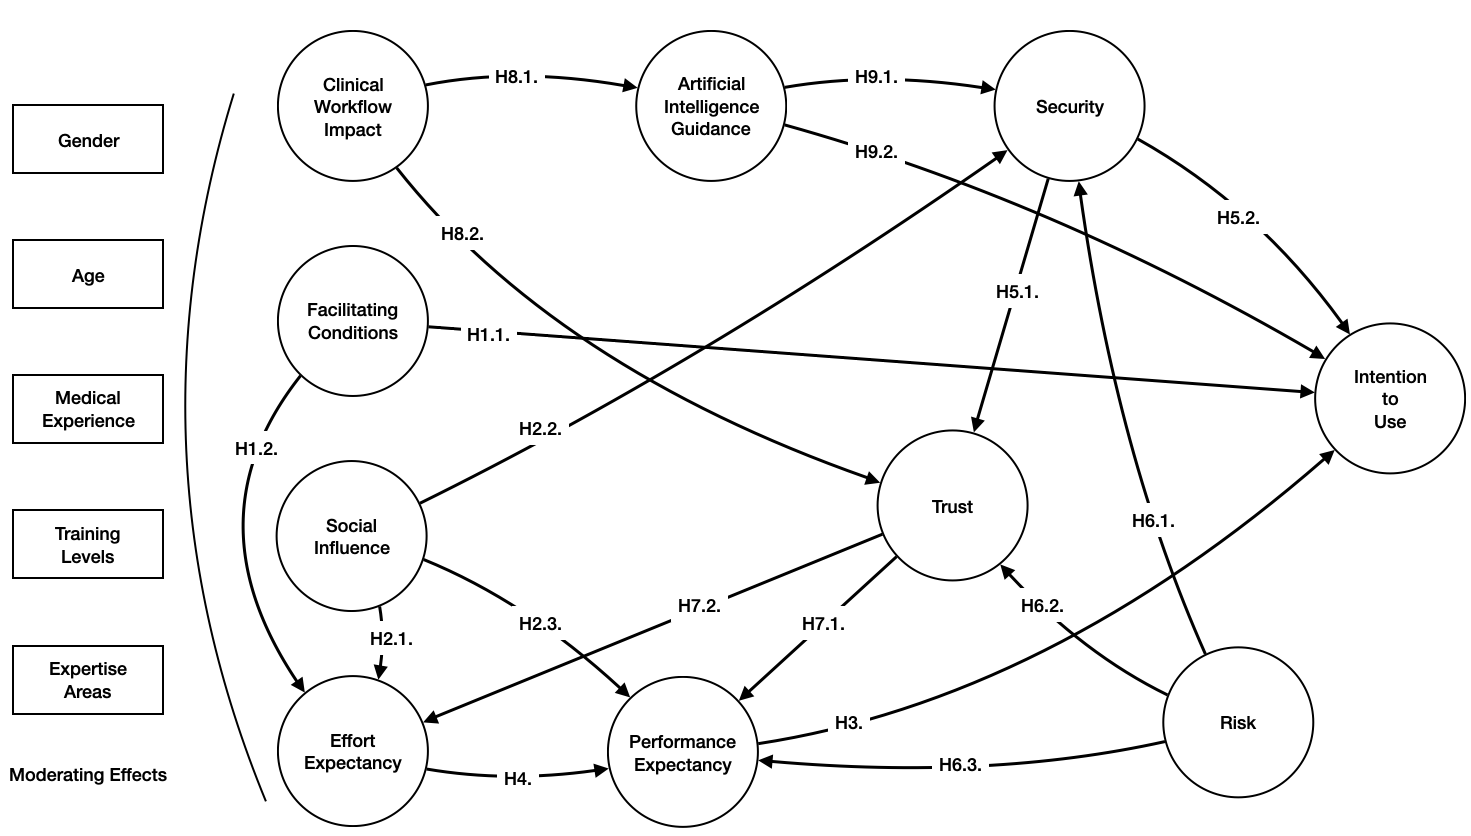
\includegraphics[width=0.885\linewidth]{fig073}
\caption{The w, comparing the relations between moderating effects, model constructs and hypotheses. We adapted this proposed research model from the UTAUT theoretical model to explain the actual adoption of AI in the medical imaging workflow. The research model includes 10 factors. We measured each factor with multiple items. Moreover, we adapted all items from extant literature to improve content validity.}
\label{fig:fig073}
\end{figure*}
%%%%%%%%%%%%%%%%%%%%%%%%%%%%%%%%%%%%%%%%%%%%%%%%%%%

This study proposes a questionnaire adapted from the UTAUT model.
Specifically, the questionnaire incorporates variables such as facilitating conditions, social influence, perceived usefulness (performance expectancy), ease of use (effort expectancy), security, risk, and trust.
To understand the relationship between variables and hypotheses, Figure~\ref{fig:fig073} presents the proposed acceptance/use model.

For testing the hypothesis, the questionnaire comprised 28 questions (items) for responses on a Likert-type scale, ranging from 1 -- ``Strongly disagree'', 2 -- ``Disagree'', 3 -- ``Undecided'', 4 -- ``Agree'', and 5 -- ``Strongly agree''.
To ensure the content validity of the questionnaire used to assess each construct, we adapted all items from previous studies regarding the measurement of the constructs~\cite{BOOTSMAN201999, LOOIJE2010386}.
We carefully reworded it to fit the context of AI applications into the medical imaging workflow.
Although this work focuses on AI applications in the medical imaging workflow, the proposed model can be generalized to other AI systems, specially in the clinical domain.

\subsection{Items Based on UTAUT Constructs}
\label{sec:chap004003001}

Based on the original UTAUT constructs, we developed several hypotheses.
Since it is newly developed, our study adopts an exploratory approach in hypothesizing the significant effects on user adoption.
Under these hypotheses, we propose a conceptual framework for the empirical study.
Not only our model covers the core determinants predicting the {\it intention to adopt} and {\it actual adoption} of AI, but it also allows the research community to analyze each moderator uncertainty that would constraint the effects of core determinants.
Because it has been empirically tested and proven superior to other models~\cite{AJZEN1991179, RePEc:inm:ormnsc:v:35:y:1989:i:8:p:982-1003}, this study chooses UTAUT as a theoretical foundation to develop the hypotheses.

\vspace{2.25mm}

\noindent
We specifically developed the following hypotheses:

\vspace{2.25mm}

{\it Facilitating Conditions}. have direct positive relations with user behavior but no effect on behavioral intentions~\cite{10.2307/30036540}.
Although other authors~\cite{KHALILZADEH2017460} are using the original UTAUT model with separate constructs, in this study we are using behavioral intention as a proxy for user behavior.

\vspace{2.25mm}

\noindent
Hence, we hypothesize that:

\vspace{2.25mm}

\noindent
{\bf H1.1.} The facilitating conditions for using AI in the clinical workflow, positively predict users' intentions to use it;

\vspace{2.25mm}

\noindent
{\bf H1.2.} The facilitating conditions ({\it e.g.}, knowledge to use the system) for using AI in the clinical workflow, has direct positive impact on effort expectancy;

\vspace{2.25mm}

{\it Social Influence}. has direct impact on behavioral intention.
The underlying assumption is that clinicians tend to consult their medical community about novel diagnosis paradigms and can be influenced by perceived social pressure.
Because perceived security also involves a patient's health for misdiagnosing the case, it should be highly influenced in the proposed model.

\vspace{2.25mm}

\noindent
Based on this, we anticipate that:

\vspace{2.25mm}

\noindent
{\bf H2.1.} The social influence ({\it e.g.}, recommendation from the medical community) for using an AI system, positively predicts effort expectancy;

\vspace{2.25mm}

\noindent
{\bf H2.2.} The social influence ({\it e.g.}, recommendation from the medical community) for using an AI system, positively and directly influences perceived security;

\vspace{2.25mm}

\noindent
{\bf H2.3.} The social influence ({\it e.g.}, recommendation from the medical community) for using an AI system, has a direct positive impact on performance expectancy;

\vspace{2.25mm}

{\it Performance Expectancy}. is the strongest predictor of behavior intention~\cite{KHALILZADEH2017460}.
Yang~\cite{Yang2010} divided the construct into two separate constructs of utilitarian performance expectancy and hedonic performance expectancy.
Although enhancing task performance could lead to increased satisfaction, some authors~\cite{ESCOBARRODRIGUEZ201470, HART201993} report a weak effect of hedonic motivation.
In radiology, one attractive goal of AI is the ability to provide an autonomous second reader to support decision-making.
Such an AI system offer utilitarian benefits that are likely to be important drivers of adoption.

\vspace{2.25mm}

\noindent
Therefore, we hypothesize that:

\vspace{2.25mm}

\noindent
{\bf H3.} Performance expectancy ({\it i.e.}, usefulness) positively affects behavioral intention to use an AI system;

{\it Effort Expectancy}. is another significant predictor of intention to use AI systems~\cite{doi:10.5465/amr.2019.0178}.
Several authors~\cite{Fan2020, Tran2021} also find effort expectancy to have a significant effect on behavioral intention.
As AI systems are providing a new shift of paradigm, it is likely that perceived degree of ease associated with AI systems will affect behavioral intention.

\noindent
In accordance, we denote that:

\vspace{2.25mm}

\noindent
{\bf H4.} Effort expectancy ({\it i.e.}, ease of use) positively affects performance expectancy ({\it i.e.}, usefulness) to use AI systems;

\subsection{Items Based on UTAUT Extensions}
\label{sec:chap004003002}

Trust, security and risk became critical additional constructs in studies about technology adoption~\cite{KHALILZADEH2017460, https://doi.org/10.1002/mar.20823}.
Specially, in the case of sharing medical information~\cite{6038852}, as clinicians are resistant to adopt new technologies~\cite{10.1145/3132272.3134111}.

\vspace{2.25mm}

{\it Perceived Security}. is expected to affect directly behavioral intention.
Because AI systems involve sensitive information about patients, it should be highly influential in the proposed model~\cite{KHALILZADEH2017460}.
Moreover, perceived security is an aggregating construct, changing over time according to the community opinion and social influence of medical experts.

\vspace{2.25mm}

\noindent
Therefore, we hypothesize that:

\vspace{2.25mm}

\noindent
{\bf H5.1.} Perceived security of AI systems positively and directly predicts perceived trust;

\vspace{2.25mm}

\noindent
{\bf H5.2.} Perceived security of AI systems positively and directly behavioral intention to use AI systems;

\vspace{2.25mm}

{\it Perceived Risk}. is usually related to perceived security.
The more a user perceives the risk, the less secure the user's feel, leading to a negative relationship between risk and security~\cite{KHALILZADEH2017460}.
Indeed, the literature~\cite{SHIN20091343, Thakur2014} states that perceived risk has negative impact on perceived security, trust, as performance expectancy.

\vspace{2.25mm}

\noindent
Based on these literature findings, we formulate the following hypothesis:

\vspace{2.25mm}

\noindent
{\bf H6.1.} The perceived risk of using AI systems has a direct negative impact on perceived security;

\vspace{2.25mm}

\noindent
{\bf H6.2.} The perceived risk of using AI systems has a direct negative impact on perceived trust;

\vspace{2.25mm}

\noindent
{\bf H6.3.} The perceived risk of using AI systems has a direct negative impact on performance expectancy;

\vspace{2.25mm}

{\it Trust}. Perceived security and trust positively affect behavioral intentions~\cite{SHIN20091343}.
As a unitary construct, the effect of trust on behavioral intention has gained notable support.
Moreover, this construct is the most significant predictor of behavioral intention~\cite{chandra2010evaluating, SHIN20091343}.
While AI-based solutions become ubiquitous, trust supersedes the importance of traditional adoption factors such as perceived usefulness.
Akin to Chandra et al.~\cite{chandra2010evaluating}, this study includes trust as a singular construct, which is likely to be critical due to the novelty of AI systems in the medical workflow and convoluted environments.

\vspace{2.25mm}

\noindent
Thus, we hypothesize that:

\vspace{2.25mm}

\noindent
{\bf H7.1.} Trust positively affects performance expectancy ({\it i.e.}, usefulness) to use AI systems;

\vspace{2.25mm}

\noindent
{\bf H7.2.} Trust positively affects effort expectancy ({\it i.e.}, ease of use) to use AI systems;

\subsection{Items Related to Impact}
\label{sec:chap004003003}

AI has a significant social and personal behavioral impact on the medical community all over the world~\cite{Fan2020}.
Medical diagnosis impacts significantly on peoples' health and peoples' lives, and clinicians have to take responsibility for their actions.
Therefore, clinicians may be more cautious than professionals in other fields when considering adopting new technologies to assist their work.
Although clinicians typically resist new technologies, several authors~\cite{doi:10.1148/ryai.2020190043, WAYMEL2019327} are reporting a new change of behavior for the adoption of AI systems in the clinical workflow, whereas these systems are increasing clinicians' performance during decision-making \cite{CALISTO2021102607}.

%%%%%%%%%%%%%%%%%%%%%%%%%%%%%%%%%%%%%%%%%%%%%%%%%%%
\begin{figure*}
\centering
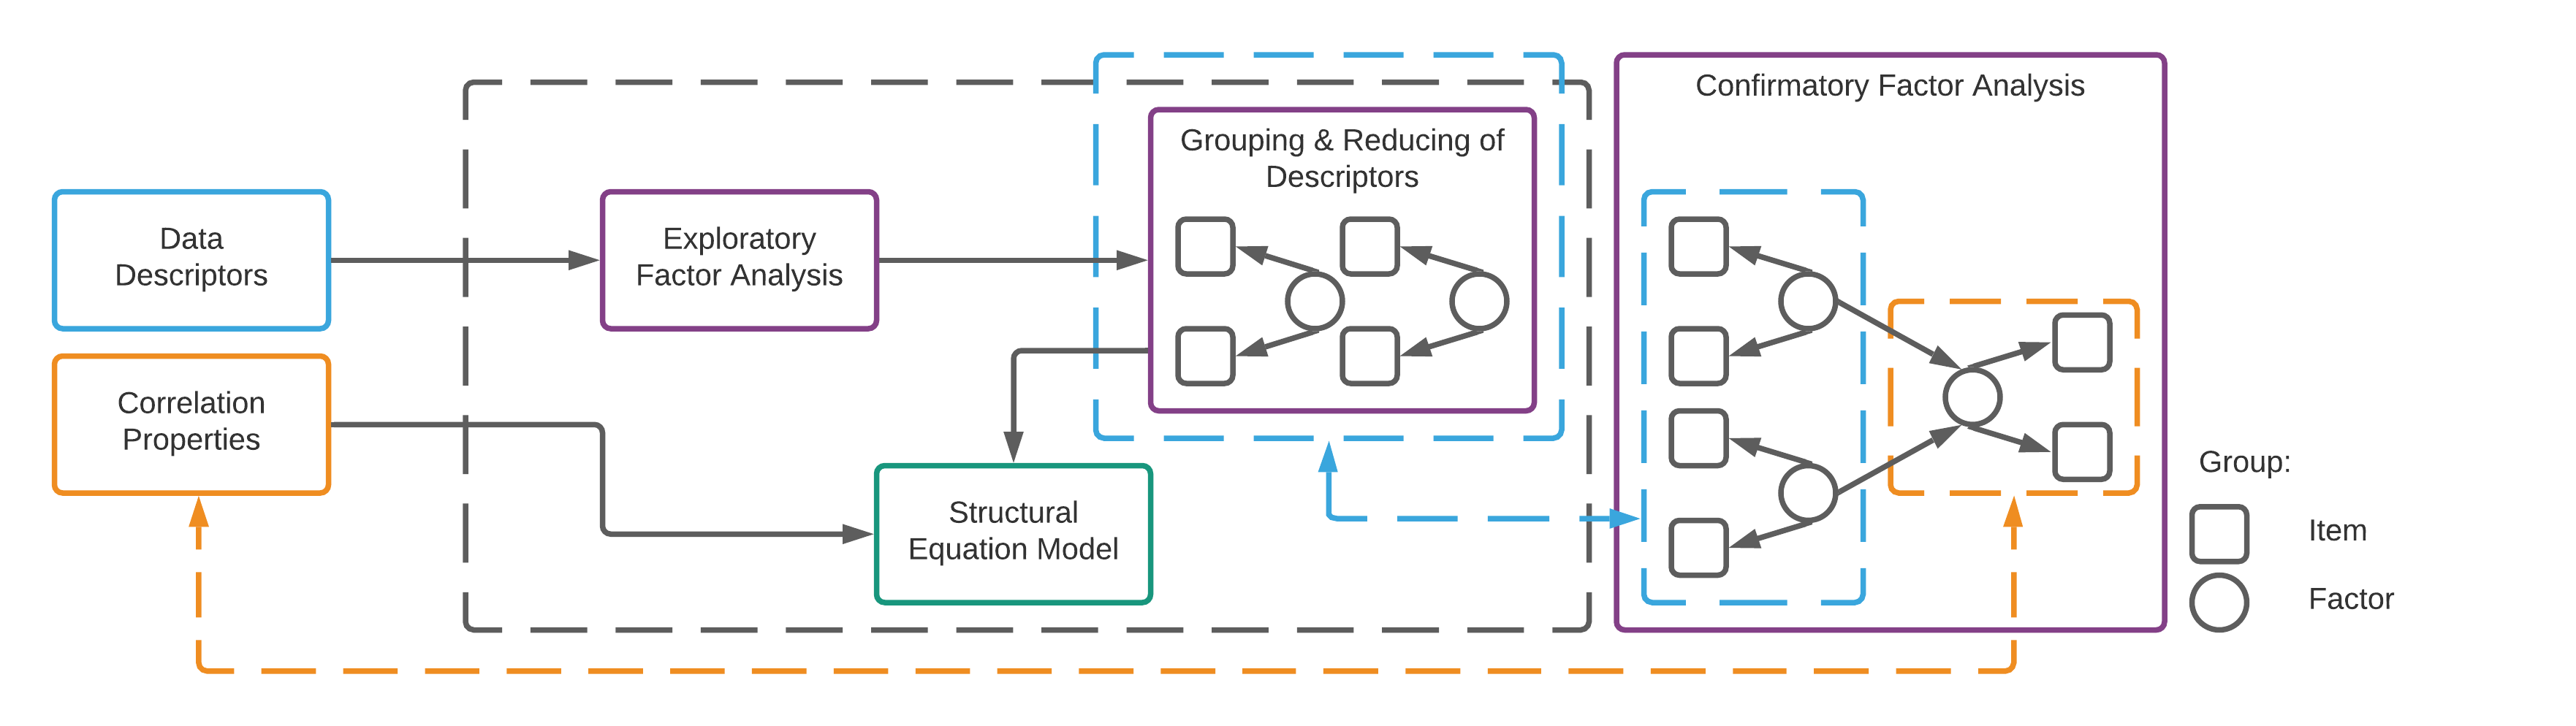
\includegraphics[width=0.985\linewidth]{fig075}
\caption{The basic statistical flow steps followed by us, which are usually taken in the framework of SEM modeling. Before the employment of the SEM modeling, we used the conceptual EFA to reduce descriptors and group them. Here, we identified the latent factors by using the CFA. Finally, we applied the SEM to estimate the coefficients.}
\label{fig:fig075}
\end{figure*}
%%%%%%%%%%%%%%%%%%%%%%%%%%%%%%%%%%%%%%%%%%%%%%%%%%%

As introduced in Section~\ref{sec:chap004002}, the TRA inspires various technology adoption models, arguing that both attitude toward an action and subjective norms have impact on behavioral intention, affecting how people perform an action~\cite{https://doi.org/10.1002/hbe2.195}.
Adapted from TRA and TAM, the UTAUT definition of attitude through behavior is ``{\it an individual's positive feeling about performing the target behavior}''~\cite{10.2307/30036540}.
On the other hand, subjective norm refers to ``{\it a person's perception that most people who are important to them think they should or should not perform the behavior in question}''~\cite{10.2307/30036540}.

\vspace{2.25mm}

\noindent
Hence, we hypothesize that:

\vspace{2.25mm}

\noindent
{\bf H8.1.} The extent to which AI positively impacts the clinical workflow ({\it e.g.}, decreasing the medical error, time-to-diagnose, etc.) due to better decision-making of clinicians, affects the intention to follow AI guidance;

\vspace{2.25mm}

\noindent
{\bf H8.2.} The extent to which AI positively impacts the clinical workflow ({\it e.g.}, decreasing the medical error, time-to-diagnose, etc.) due to better decision-making of clinicians, directly predicts perceived trust;

\vspace{2.25mm}

Salient beliefs and evaluations determine a person's attitude toward a behavior~\cite{KHALILZADEH2017460}.
In fact, several studies report a strong relationship between trust, risk, and behavior intentions~\cite{GANSSER2021101535, 9197782, https://doi.org/10.1002/mar.20823}.
Although trust and perceived risk significantly affect behavioral intention, in some of these studies, trust negatively affects perceptions of risk.
When it comes to applications that require context awareness~\cite{10.1145/3313831.3376506}, as it involves machines to learn subjective data, clinicians have significant concerns about trusting AI.

Existing studies have not explicitly examined whether perceived risk plays a mediating role~\cite{AMEEN2021106548}.
As clinicians are likely to perceive AI guidance as being highly risky for patients, trust will likely play a significant role in behavioral intention than perceived risk.
Instead, its role will be more critical in reducing risk perceptions for misdiagnosing a patient.

\noindent
Given the wide applicability of UTAUT, we can anticipate that:

\vspace{2.25mm}

\noindent
{\bf H9.1.} The willingness to follow the AI guidance positively and directly influences perceived security;

\vspace{2.25mm}

\noindent
{\bf H9.2.} The willingness to follow the AI guidance positively affects intention to use AI systems;

\section{Methods}
\label{sec:chap004004}

Our research model includes ten constructs.
For this study, we measured each construct with multiple items (Figure~\ref{fig:fig075}).
To preserve the content validity and reliability, we measured most of our items from the extant literature~\cite{SOHN2020101324, info:doi/10.2196/14316}.
Finally, we adjusted these items in our questionnaire to match the context of AI adoption among clinicians.

In compliance with recommendations of the two-stage analytical procedure, we used Confirmatory Factor Analysis (CFA) to test the measurement model’s validity and reliability~\cite{2019-07124-034}.
In addition, we used Structural Equation Modeling (SEM) as a preferable technique to regression. It allows simultaneous analysis of all relationships through multiple regression while also allowing for both observed and latent variables to be analyzed simultaneously and providing overall fit statistics.

We conducted CFA using the \texttt{R language} (\texttt{v 4.0.2}) employing Maximum Likelihood Estimation (MLE).
Furthermore, MLE was then followed by path analysis of the structural relationships conducted in the \texttt{R language} with SEM libraries (\texttt{lavaan v. 0.6-7} and \texttt{semTools v. 0.5-3}).
We also undertook moderation analysis in the \texttt{R language}.

\subsection{Procedures}
\label{sec:chap004004001}

We sent the questionnaire via social media ({\it e.g.}, radiology groups on Facebook and LinkedIn) to 17203 participants who gave prior permission to use their data for research purposes under this international study.
The questionnaire contained i) a general explanation of the study, ii) the details of the privacy policy, iii) data treatment, and a iv) link to a Google Forms survey.

We sent the questionnaire in the middle of February 2021.
The criterion was to send the questionnaire to clinicians worldwide who are members of these social media target groups ({\it i.e.}, radiologists, physicians from any other expertise, technicians, etc.).
Overall, this procedure remained until the end of July 2021, when we analysed and discussed our data.

\subsection{Participants}
\label{sec:chap004004002}

Table~\ref{tab:tab008} is listing the sample demographics under this study.
In total, we collected data from 322 participants, corresponding to an overall participation of 1.9\%.
The participation was higher from people of the USA/Canada (25.5\%), Africa (11.2\%), Portugal (10.6\%), and Other-EU Countries (9.9\%).
On the other hand, the participation was lower from the Middle East (8.1\%), Asia (7.5\%), South or Central America (5.9\%), Italy (5.3\%), UK (4.3\%), Non-EU European (3.7\%), New Zealand/Australia (2.8\%), France (1.9\%), Germany (1.9\%), and Spain (1.6\%).

Regarding general demographics (N = 322), the sample consisted of a slightly higher proportion of men (59.9\%) than women (38.8\%) with 1.2\% answering ``Prefer not to say''.
For age groups, 12.1\% of participants range from 18 to 29 years old, 29.5\% from 30 to 39, 22.7\% from 40 to 49, 23.9\% from 50 to 59, 10.2\% older than 59, and 1.6 answering ``Prefer not to say''.

%%%%%%%%%%%%%%%%%%%%%%%%%%%%%%%%%%%%%%%%%%%%%%%%%%%
\begin{table}[htpb]
\resizebox{\columnwidth}{!}{%
\begin{tabular}{cccc}
\hline
\rule{0mm}{4mm}
Demographic                   & Group                    & Frequency & Percentage
\\
\hline
\multirow[t]{3}{*}{Gender}       & Female                    & 125       & 38.8\%     \\
                                 & Male                      & 193       & 59.9       \\
                                 & Other                     & 4         & 1.2        \\
\hline
\multirow[t]{6}{*}{Age}          & 18 - 29                  & 39        & 12.1\%     \\
                                 & 30 - 39                  & 95        & 29.5\%     \\
                                 & 40 - 49                  & 73        & 22.7\%     \\
                                 & 50 - 59                  & 77        & 23.9\%     \\
                                 & > 59                     & 33        & 10.2\%     \\
                                 & N.A.                     & 5         & 1.6\%      \\
\hline
\multirow[t]{7}{*}{Nationality}  & Europe                   & 126       & 39.2\%     \\
                                 & North America            & 82        & 25.5\%     \\
                                 & Africa                   & 36        & 11.2\%     \\
                                 & Middle East              & 26        & 8.1\%      \\
                                 & Asia                     & 24        & 7.5\%      \\
                                 & Central \& South America & 19        & 5.9\%      \\
                                 & Oceania                  & 9         & 2.8\%      \\
\hline
\multirow[t]{5}{*}{Education}    & Specialists              & 111       & 34.5\%     \\
                                 & Bachelor                 & 81        & 25.2\%     \\
                                 & Master                   & 78        & 24.2\%     \\
                                 & PhD                      & 45        & 14\%       \\
                                 & N.A.                     & 7         & 2.1\%      \\
\hline
\multirow[t]{5}{*}{Medical Experience} & Interns            & 24        & 7.5\%      \\
                                       & Juniors            & 26        & 8.1\%      \\
                                       & Middles            & 54        & 16.5\%     \\
                                       & Seniors            & 210       & 65.2\%     \\
                                       & N.A.               & 8         & 2.4\%      \\
\hline
\multirow[t]{3}{*}{Training Levels}    & Doctors            & 132       & 41\%       \\
                                       & Technicians        & 105       & 32.6\%     \\
                                       & Other              & 85        & 26.4\%     \\
\hline
\end{tabular}%
}
\caption{Characteristics of participants for demographic groups with frequency and percentage. The main characteristics are gender, age, nationality, and education.}
\label{tab:tab008}
\end{table}
%%%%%%%%%%%%%%%%%%%%%%%%%%%%%%%%%%%%%%%%%%%%%%%%%%%

Other demographic data are important to this study, such as medical experience of participants (Section~\ref{sec:chap004004002001}), training levels (Section~\ref{sec:chap004004002002}), and expertise areas (Section~\ref{sec:chap004004002003}).
In this study, the education level of participants is also important to denote relations between demographic data.
Specifically, 34.5\% of participants are specialists, 25.2\% have at least one bachelor degree, 24.2\% have a master degree, and 14\% a PhD.
The other 2.1\% are typically students or academic associate degrees.

\subsubsection{Medical Experience}
\label{sec:chap004004002001}

Concerning medical experience, 65.2\% are seniors with more than 10 years of experience.
Additionally, 16.5\% are middles with more than 5 years of work but less than 10 years.
Clustering both categories together, this makes a total of 81.7\% clinical experts.
On the contrary, 8.1\% are juniors up to 5 years after taking the exam.
Besides, 7.5\% are interns before the specialty exam.
Within these two groups, we clustered the information, making a total of 15.6\% clinical novices.
The other 2.4\% are students and academics who do not considered any of the above groups.

\subsubsection{Training Levels}
\label{sec:chap004004002002}

For the training levels, 41\% of participants are doctors, 32.6\% are technicians, and 26.4\% received different training, such as nursing, medical physics or biomedical sciences, but are working on medical imaging.
To understand the procedures of the clinical workflow, information about the work sector of each participant is also important.
Under this purpose, we also analyzed the work sector, where 17.39\% work on both Public/Private sectors, 39.41\% of participants work only on the public sector (such as public hospitals or public cancer institutes), 32.91\% work only on the private sector (such as private clinics or private hospitals), and the other 10.29\% are working for companies ({\it e.g.}, medical devices), are academics or retired.

\subsubsection{Expertise Areas}
\label{sec:chap004004002003}

Finally, for the expertise areas, 79.2\% of participants work in the radiology field.
For this study, it is also important to analyze other expertise areas, as some of these categories work in medical imaging.
For instance, 7.1\% of participants work in medical intervention, 5.6\% in oncology, and 4.3\% in general medicine.
With lower participation, but still important to report, 2.5\% of participants work in surgery, 2.2\% in family medicine, and 1.6\% in several other categories.

\section{Results}
\label{sec:chap004005}

The results of the sample characteristics (Table~\ref{tab:tab008}) indicate that a typical participant of this study was a male radiology specialist between 30 and 39 years old, considered seniors with more than ten years of experience.
The primary working place was in the public sector.
We ask participants how often and how long they analyze medical imaging exams.
Specifically, 66.1\% answered they do analyze patients with medical imaging exams every day, 7.8\% answered 3 or 4 days a week, 3.7\% answered 2 or 3 days a week, another 3.7\% answered once a week. The other 18.7\% answered monthly or as needed.

Regarding how long they analyze patients with medical imaging exams, 28\% answered more than 20 years, 27\% with less than five years, 17.1\% between 6 and 10 years, 15.5\% between 11 and 15 years, and finally, 12.4\% between 16 and 20 years.
Moreover, we gave participants additional questions about their experience with AI systems and the frequency of their use.
Respectively, 42.5\% answered they know about AI but never tried it, 27\% have attempted to but do not use it regularly, 19.3\% use it regularly, and 11.2\% never heard about AI systems.

\subsection{Checking Assumptions}
\label{sec:chap004005001}

We checked the SEM assumptions, where all variables showed a normal distribution based on a visual inspection of box plots and histograms.
Residuals showed a normal distribution with no relation between residuals and predictors~\cite{murtagh2012multivariate}.
The overall fit of the model was good, with all the relevant goodness of fit indices higher than the recommended threshold of 0.90 for adjusted goodness of fit indices and 0.95 for other indices~\cite{Bagozzi2012, doi:10.1504/IJMDA.2017.087624, murtagh2012multivariate, SUMAK2016602}.

Under this study, the Goodness of Fit Index (GFI) = 0.824, the Adjusted Goodness of Fit Index (AGFI) was 0.784, the Comparative Fit Index (CFI) = 0.909, the Normative Fit Index (NFI) was 0.861, and the Tucker-Lewis Index (TLI) = 0.896 reported from our analysis.
Although goodness of fit ($GFI = 0.824 < 0.90$), adjusted goodness of fit ($AGFI = 0.784 < 0.80$), and Tucker-Lewis test ($TLI = 0.896 < 0.90$) are slightly lower than the recommended levels, studies have shown that sample size impacts these fit indices~\cite{KHALILZADEH2017460, doi:10.1080/00273171.2019.1602503, ZHOU2010760}.
Some of these studies show the downward bias of the previously mentioned indices when the degree of freedom values increase in comparison to the sample size of the model~\cite{doi:10.1080/00273171.2019.1602503}.
Indeed, the ratio of the test statistic ($\chi^2$) to the degree of freedom ($df$) was lower than 3.0 as recommended ($\chi^2$ / $df$ $= 2.587 < 3.0$) in the literature.
Pairwise with the Root Mean Square of Error Approximation ($RMSEA = 0.073 < 0.08$), both indicated an acceptable model fit~\cite{ZHOU2010760}.

The test statistic ($\chi^2$) for the model was significant due to the sample size.
Based on Hoelter index~\cite{https://doi.org/10.1002/nur.20088}, the sample size of 138 is sufficient and the sample of 322 seems adequate for the sophisticated model of the study.
Additionally, the Standardized Root Mean Square Residual (SRMR) was also good, at 0.083, above the threshold ($SRMR = 0.083 > 0.06$) for a good overall fit.

\subsection{Measurement Model}
\label{sec:chap004005002}

Given the satisfactory measurement of the model fit, we initiated measuring each construct (Section~\ref{sec:chap004005002}).
From here, we aim to purify the measurement items, to check the model fit, validity, and reliability of the measurement scales.
Thoroughly, Table~\ref{tab:tab009} reports the results of the CFA.

%%%%%%%%%%%%%%%%%%%%%%%%%%%%%%%%%%%%%%%%%%%%%%%%%%%
\begin{table*}
\resizebox{\textwidth}{!}{%
\begin{tabular}{ccccccccccc}
\hline
Measure & Impact & Guidance & PerfExp & EffExp & SocInf & FacCond & IntUse & Security & Risk & Trust \\ \hline
alpha   & 0.57   & 0.88     & 0.87    & 0.89   & 0.73   & 0.80    & 0.94   & 0.83     & 0.84    & 0.88  \\
CR      & 0.57   & 0.88     & 0.89    & 0.89   & 0.74   & 0.79    & 0.93   & 0.82     & 0.84    & 0.88  \\
AVE     & 0.40   & 0.65     & 0.72    & 0.73   & 0.49   & 0.55    & 0.78   & 0.60     & 0.64    & 0.70  \\ \hline
\end{tabular}%
}
\caption{The abbreviated constructs are as follows: Clinical Workflow Impact (Impact); AI Guidance (Guidance); Performance Expectancy (PerfExp); Effort Expectancy (EffExp); Social Influence (SocInf); Facilitating Conditions (FacCond); Behavior Intention to Use (IntUse); Perceived Security (Security); Perceived Risk (Risk); Perceived Trust (Trust). Moreover, the measure abbreviations are: Cronbach alpha (alpha); Composite Reliability (CR); Average Variance Extracted (AVE).}
\label{tab:tab009}
\end{table*}
%%%%%%%%%%%%%%%%%%%%%%%%%%%%%%%%%%%%%%%%%%%%%%%%%%%

Convergent validity shows whether each factor can be reflected by its items~\cite{10.3389/fpubh.2018.00149, Henseler2015}.
To this end, all loadings were significant at alpha level ({\it p-value} = 0.000), and the minimum loading was 0.57, with most loadings higher than 0.8, which indicates good convergent validity~\cite{info:doi/10.2196/14316}.
Each item loaded significantly ({\it p-value} < 0.001) on its underlying construct in all cases.
On the other hand, discriminant validity reflects whether two factors are statistically different~\cite{10.3389/fpubh.2018.00149, Henseler2015}.
For that, we examined both convergence and discriminant validity of the model, measuring the reliability of each measure and each construct and the Average Variance Extracted (AVE) for each construct.

We compared the shared variance across constructs with the AVE from the individual construct to examine discriminant validity.
The shared variety between constructs was lower than the AVE from the individual constructs (Table~\ref{tab:tab009}), confirming discriminant validity.
In the end, we checked the measurement model for the Composite Reliability ($CR = 0.95$), which indicated good measurement reliability of our measurement model~\cite{Bagozzi2012, doi:10.1504/IJMDA.2017.087624, murtagh2012multivariate, SUMAK2016602}.

To conclude, the measurement model demonstrated adequate reliability, convergent validity, and discriminant validity.
However, given the complex relationships across the model's factors, we should consider the moderating effects on other variables.
Expressly, we can reasonably assume that the model has unexpected moderating relationships.
Hence, the recognition of moderating effects for demographics (Section~\ref{sec:chap004005004}) across the factors is particularly important in this study and must be further reported.

\subsection{Parallel Analysis}
\label{sec:chap004005006}

To measure how many factors should we keep, we must base that on multiple pieces of information, such as parallel analysis~\cite{doi:10.1080/10705511.2019.1615835}.
Parallel analysis is a simulation based on the number of items {\it vs.} sample size, while computing the simulated eigenvalues, which can be used to compare the eigenvalues from the analysis (Figure~\ref{fig:fig093}).
Specifically, it indicates if there are factors with dots overlap between the eigenvalue sizes and the cut off-line for the retention.

Large changes in effect size indicate a break point for the number of factors, but we also must consider the line limits of the parallel analysis.
For instance, the difference between the first components can sustain the argument for choosing the optimal eigenvalue size as four (Figure~\ref{fig:fig093}).
However, we can also observe that this difference is much more conclusive for the comparison between the components five and six, as well as between the six and seven.
Where both components eight and night are almost totally below the line, the rule for keeping an item for a factor or overall are generally arbitrary~\cite{doi:10.1207/S15328031US0201}.

%%%%%%%%%%%%%%%%%%%%%%%%%%%%%%%%%%%%%%%%%%%%%%%%%%%
\begin{figure}
\centering
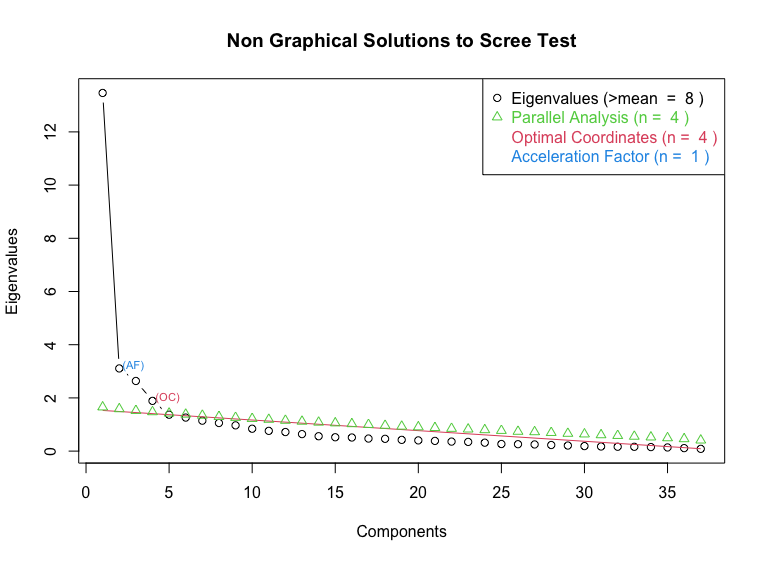
\includegraphics[width=0.985\linewidth]{fig093}
\caption{Scree plot of eigenvalues with the eigenvalues greater than one rule, elbow bend, and intersecting lines.}
\label{fig:fig093}
\end{figure}
%%%%%%%%%%%%%%%%%%%%%%%%%%%%%%%%%%%%%%%%%%%%%%%%%%%

\subsection{Structural Model}
\label{sec:chap004005003}

Since the measurement model achieves an overall fit, we used SEM to analyze our data.
Structural modeling evaluates whether data fits the theoretical measurement of the model~\cite{doi:10.1080/10705511.2017.1401932}.
This study extends the proposed research model to include two new constructs:
(1) Clinical Workflow Impact; and
(2) AI Guidance.
Additionally, we extended the two constructs to new interactions between these constructs and security, trust, and behavioral intention to use.
To test the structural relationships, we estimated the hypothesized casual paths (Figure~\ref{fig:fig073}).
From Table~\ref{tab:tab011}, we can denote that the study supports ({\it p-value} < 0.10) the majority of hypotheses, except for {\bf H6.1}, {\bf H6.3}, and {\bf H7.1} hypotheses.

The coefficient of determination ($R^2$), also known as Squared Multiple Correlations (SMC), was calculated for the constructs of the measurement model (Table~\ref{tab:tab010}).
This coefficient varies between 0 and 1, while indicating the explanatory power of the model and predictive accuracy~\cite{doi:10.1080/10705511.2017.1401932}.
It shows the portion of the total variance in the dependent variable that can be accounted for by the independent variables.

Higher loadings indicate that items are strongly related to the latent variables.
In addition, the $R^2$ values express the variance of items explained by the latent factor (Table~\ref{tab:tab010}).
The $R^2$ values are the squared factor loadings extracted from the CFA model.

%%%%%%%%%%%%%%%%%%%%%%%%%%%%%%%%%%%%%%%%%%%%%%%%%%%
\begin{table}[htpb]
\resizebox{\columnwidth}{!}{%
\begin{tabular}{llrrrl}
\hline
Construct                   & Item        & \multicolumn{1}{l}{Alpha} & \multicolumn{1}{l}{StdError} & \multicolumn{1}{l}{z-value} & p-value \\ \hline
Clinical Workflow Impact & Impact\_1   & 0.53 & 0.080 & 6.615  & 0.000 \\
Alpha = 0.57                & Impact\_2   & 0.75  & 0.079    & 9.499   & 0.000   \\ \hline
AI Guidance              & Guidance\_1 & 0.36 & 0.035 & 10.209 & 0.000 \\
Alpha = 0.88             & Guidance\_2 & 0.29 & 0.028 & 10.102 & 0.000 \\
R2 = 0.238                  & Guidance\_3 & 0.19  & 0.026    & 7.262   & 0.000   \\
                            & Guidance\_4 & 0.32  & 0.033    & 9.683   & 0.000   \\ \hline
Performance Expectancy      & PerfExp\_1  & 0.45                      & 0.039                        & 11.606                      & 0.000   \\
Alpha = 0.87                & PerfExp\_2  & 0.14                      & 0.019                        & 7.186                       & 0.000   \\
R2 = 0.595                  & PerfExp\_3  & 0.08                      & 0.018                        & 4.382                       & 0.000   \\ \hline
Effort Expectancy           & EffExp\_1   & 0.16                      & 0.022                        & 7.335                       & 0.000   \\
Alpha = 0.89                & EffExp\_2   & 0.19                      & 0.021                        & 8.615                       & 0.000   \\
R2 = 0.496                  & EffExp\_3   & 0.25                      & 0.025                        & 9.821                       & 0.000   \\ \hline
Social Influence            & SocInf\_1   & 0.57                      & 0.054                        & 10.464                      & 0.000   \\
Alpha = 0.73                & SocInf\_2   & 0.68                      & 0.066                        & 10.24                       & 0.000   \\
                            & SocInf\_3   & 0.35                      & 0.047                        & 7.356                       & 0.000   \\ \hline
Facilitating Conditions     & FacCond\_1  & 0.56                      & 0.06                         & 9.284                       & 0.000   \\
Alpha = 0.80                & FacCond\_2  & 0.57                      & 0.061                        & 9.45                        & 0.000   \\
                            & FacCond\_3  & 0.41                      & 0.046                        & 8.932                       & 0.000   \\ \hline
Behavioral Intention to Use & IntUse\_1   & 0.16                      & 0.017                        & 9.576                       & 0.000   \\
Alpha = 0.94                & IntUse\_2   & 0.13                      & 0.015                        & 8.496                       & 0.000   \\
R2 = 0.681                  & IntUse\_3   & 0.15                      & 0.016                        & 9.761                       & 0.000   \\
                            & IntUse\_4   & 0.19                      & 0.019                        & 9.856                       & 0.000   \\ \hline
Security                    & Security\_1 & 0.41                      & 0.041                        & 10.055                      & 0.000   \\
Alpha = 0.83                & Security\_2 & 0.14                      & 0.025                        & 5.621                       & 0.000   \\
R2 = 0.397                  & Security\_3 & 0.39                      & 0.037                        & 10.537                      & 0.000   \\ \hline
Risk                        & Risk\_1  & 0.36                         & 0.049                        & 7.342                       & 0.000   \\
Alpha = 0.84                & Risk\_2  & 0.57                         & 0.06                         & 9.48                        & 0.000   \\
                            & Risk\_3  & 0.34                         & 0.047                        & 7.114                       & 0.000   \\ \hline
Trust                       & Trust\_1    & 0.30                      & 0.031                        & 9.762                       & 0.000   \\
Alpha = 0.88                & Trust\_2    & 0.19                      & 0.025                        & 7.606                       & 0.000   \\
R2 = 0.465                  & Trust\_3    & 0.21                      & 0.029                        & 7.385                       & 0.000  \\ \hline
\end{tabular}%
}
\caption{The measuring model with: Clinical Workflow Impact ({\bf Impact}); AI Guidance ({\bf Guidance}); Performance Expectancy ({\bf PerfExp}); Effort Expectancy ({\bf EffExp}); Social Influence ({\bf SocInf}); Facilitating Conditions ({\bf FacCond}); Behavioral Intention to Use ({\bf IntUse}); {\bf Security}; {\bf Risk}; and {\bf Trust}. The computed measurements are {\bf Alpha}, Standard Error ({\bf StdError}), {\bf z-value}, and {\bf p-value}.}
\label{tab:tab010}
\end{table}
%%%%%%%%%%%%%%%%%%%%%%%%%%%%%%%%%%%%%%%%%%%%%%%%%%%

The $R^2$ of the behavioral intention was the highest at 0.681 (Table~\ref{tab:tab010}), which showed that the proposed model explained a considerable amount of the variance for the dependent variable.
The lowest amount of $R^2$ in the model belongs to AI Guidance ($R^2$ = 0.238), followed by security ($R^2$ = 0.397), due to their proximity to independent variables, as well as the nature of the constructs, which are rooted in terms of a clinician's belief in AI systems.
The coefficient for performance expectancy ($R^2$ = 0.595), effort expectancy ($R^2$ = 0.496), and trust ($R^2$ = 0.465) were also acceptable, which is consistent with previous results~\cite{KHALILZADEH2017460}.

\subsection{Moderating Effects}
\label{sec:chap004005004}

To investigate demographic moderator effects, we conducted a moderating analysis using the split sample approach \cite{LI2021106581, LI2021106929}.
This approach uses a pre-established moderator level, which emerges naturally from data and cannot be modified by the study.
For instance, the nationality of a clinician, gender, or age variables is a form of different moderator levels.
We tested the moderator effects of gender (F/M), age (divided into two groups $<$ 30 and $\geq$ 30), nationality (grouped into developed and developing countries), education (higher and advanced education), and a proxy of clinical knowledge (expert {\it vs.} novice) for working with medical imaging technologies, which was calculated from a combination of medical experience (Section~\ref{sec:chap004004002001}), training levels (Section~\ref{sec:chap004004002002}), and expertise areas (Section~\ref{sec:chap004004002003}).

We classified senior and middle radiology doctors as experts working with medical imaging technologies.
Similarly, we also consider senior and middle radiology technicians as an expert with knowledge of working with these technologies.
On the contrary, we consider novice knowledge all juniors and interns independently of being doctors, technicians, or another different training level.
We also considered all clinicians not working directly in radiology expertise as novice knowledge of working with medical imaging technologies.

%%%%%%%%%%%%%%%%%%%%%%%%%%%%%%%%%%%%%%%%%%%%%%%%%%%
\begin{table}[htpb]
\resizebox{\columnwidth}{!}{%
\begin{tabular}{lrrrrrl}
\hline
Hypotheses & \multicolumn{1}{l}{b} & \multicolumn{1}{l}{StdError} & \multicolumn{1}{l}{z-value} & \multicolumn{1}{l}{p-value} & \multicolumn{1}{l}{beta} & Supported \\
\hline
\textbf{H1.1.} & 0.313  & 0.053 & 5.912  & 0.000 & 0.349  & Yes ***                  \\
\textbf{H1.2.} & 0.432  & 0.08  & 5.393  & 0.000 & 0.375  & Yes ***                  \\
\textbf{H2.1.} & 0.268  & 0.133 & 2.015  & 0.044 & 0.211  & Yes **                   \\
\textbf{H2.2.} & 0.432  & 0.08  & 5.393  & 0.000 & 0.375  & Yes ***                  \\
\textbf{H2.3}  & 0.239  & 0.067 & 3.554  & 0.000 & 0.243  & Yes ***                  \\
\textbf{H3.}   & 0.327  & 0.068 & 4.81   & 0.000 & 0.264  & Yes ***                  \\
\textbf{H4.}   & 0.466  & 0.061 & 7.653  & 0.000 & 0.603  & Yes ***                  \\
\textbf{H5.1.} & 0.701  & 0.078 & 9.012  & 0.000 & 0.715  & Yes ***                  \\
\textbf{H5.2.} & 0.239  & 0.06  & 4.005  & 0.000 & 0.226  & Yes ***                  \\
\textbf{H6.1.} & -0.016 & 0.049 & -0.326 & 0.744 & -0.02  & \textcolor{red}{No}      \\
\textbf{H6.2.} & -0.098 & 0.059 & -1.672 & 0.095 & -0.124 & Yes *                    \\
\textbf{H6.3.} & -0.031 & 0.033 & -0.962 & 0.336 & -0.046 & \textcolor{red}{No}      \\
\textbf{H7.1.} & 0.009  & 0.045 & 0.197  & 0.844 & 0.01   & \textcolor{red}{No}      \\
\textbf{H7.2.} & 0.375  & 0.062 & 6.014  & 0.000 & 0.333  & Yes ***                  \\
\textbf{H8.1.} & -0.494 & 0.09  & -5.512 & 0.000 & -0.487 & Yes ***                  \\
\textbf{H8.2.} & 0.176  & 0.092 & 1.92   & 0.055 & 0.179  & Yes *                    \\
\textbf{H9.1.} & 0.459  & 0.067 & 6.861  & 0.000 & 0.464  & Yes ***                  \\
\textbf{H9.2.} & 0.336  & 0.055 & 6.151  & 0.000 & 0.322  & Yes ***                  \\
\hline
\end{tabular}%
}
\caption{Summary of hypothesis tests. The variables assigned to the significance values are as follows: *** significant at level $\alpha = 0.01$; ** significant at level $\alpha = 0.05$; and * significant fixed at level $\alpha = 0.10$.}
\label{tab:tab011}
\end{table}
%%%%%%%%%%%%%%%%%%%%%%%%%%%%%%%%%%%%%%%%%%%%%%%%%%%

We tested the moderating effects (Table~\ref{tab:tab012}) of the above variables by comparing, between the different groups, the path coefficients produced for each moderator after testing for measurement invariance using $X^2$ difference tests, and the fit indices.
Furthermore, we tested invariance for factor structure, loading, residuals, and means.
The model supported enough evidence of measurement invariance at {\it p-value} < 0.001 significance.

%%%%%%%%%%%%%%%%%%%%%%%%%%%%%%%%%%%%%%%%%%%%%%%%%%%
\begin{table}[htpb]
\resizebox{\textwidth}{!}{%
\begin{tabular}{|l|ll|ll|ll|ll|ll|}
\hline
\multicolumn{1}{|c|}{\multirow{2}{*}{Hypotheses}} &
  \multicolumn{2}{c|}{Gender} &
  \multicolumn{2}{c|}{Age} &
  \multicolumn{2}{c|}{Nationality Classification} &
  \multicolumn{2}{c|}{Education} &
  \multicolumn{2}{c|}{Knowledge} \\ \cline{2-11} 
\multicolumn{1}{|c|}{} &
  \multicolumn{1}{c|}{Woman} &
  \multicolumn{1}{c|}{Man} &
  \multicolumn{1}{c|}{\textless 30} &
  \multicolumn{1}{c|}{\textgreater{}= 30} &
  \multicolumn{1}{c|}{Developed} &
  \multicolumn{1}{c|}{Developing} &
  \multicolumn{1}{c|}{Higher} &
  \multicolumn{1}{c|}{Advanced} &
  \multicolumn{1}{c|}{Expert} &
  \multicolumn{1}{c|}{Novice} \\ \hline
\textbf{H1.1.} &
  \multicolumn{1}{l|}{$\textcolor{red}{\downarrow}$ 0.39 ***} &
  $\textcolor{blue}{\uparrow}$ 0.64 *** &
  \multicolumn{1}{l|}{$\textcolor{red}{\downarrow}$ 0.09 \textcolor{red}{ns}} &
  0.57 *** &
  \multicolumn{1}{l|}{$\textcolor{red}{\downarrow}$ 0.59 ***} &
  $\textcolor{red}{\downarrow}$ 0.36 *** &
  \multicolumn{1}{l|}{0.53 ***} &
  $\textcolor{red}{\downarrow}$ 0.33 *** &
  \multicolumn{1}{l|}{0.59 ***} &
  $\textcolor{red}{\downarrow}$ 0.23 ** \\ \hline
\textbf{H1.2.} &
  \multicolumn{1}{l|}{$\textcolor{red}{\downarrow}$ 0.36 ***} &
  $\textcolor{blue}{\uparrow}$ 0.61 *** &
  \multicolumn{1}{l|}{$\textcolor{red}{\downarrow}$ 0.09 \textcolor{red}{ns}} &
  $\textcolor{blue}{\uparrow}$ 0.59 *** &
  \multicolumn{1}{l|}{$\textcolor{red}{\downarrow}$ 0.47 ***} &
  $\textcolor{red}{\downarrow}$ 0.33 *** &
  \multicolumn{1}{l|}{0.51 ***} &
  $\textcolor{red}{\downarrow}$ 0.26 *** &
  \multicolumn{1}{l|}{$\textcolor{blue}{\uparrow}$ 0.59 ***} &
  $\textcolor{red}{\downarrow}$ 0.12 \textcolor{red}{ns} \\ \hline
\textbf{H2.1.} &
  \multicolumn{1}{l|}{$\textcolor{blue}{\uparrow}$ 0.38 ***} &
  $\textcolor{blue}{\uparrow}$ 0.54 *** &
  \multicolumn{1}{l|}{$\textcolor{red}{\downarrow}$ 0.11 \textcolor{red}{ns}} &
  $\textcolor{blue}{\uparrow}$ 0.56 *** &
  \multicolumn{1}{l|}{$\textcolor{blue}{\uparrow}$ 0.39 ***} &
  $\textcolor{blue}{\uparrow}$ 0.41 *** &
  \multicolumn{1}{l|}{$\textcolor{blue}{\uparrow}$ 0.47 ***} &
  $\textcolor{blue}{\uparrow}$ 0.35 *** &
  \multicolumn{1}{l|}{$\textcolor{blue}{\uparrow}$ 0.56 ***} &
  $\textcolor{red}{\downarrow}$ 0.15 \textcolor{red}{ns} \\ \hline
\textbf{H2.2.} &
  \multicolumn{1}{l|}{$\textcolor{red}{\downarrow}$ 0.27 **} &
  0.54 *** &
  \multicolumn{1}{l|}{$\textcolor{red}{\downarrow}$ 0.11 \textcolor{red}{ns}} &
  0.56 *** &
  \multicolumn{1}{l|}{$\textcolor{red}{\downarrow}$ 0.35 ***} &
  $\textcolor{red}{\downarrow}$ 0.36 *** &
  \multicolumn{1}{l|}{0.47 ***} &
  $\textcolor{red}{\downarrow}$ 0.24 ** &
  \multicolumn{1}{l|}{0.49 ***} &
  $\textcolor{red}{\downarrow}$ 0.15 \textcolor{red}{ns} \\ \hline
\textbf{H2.3} &
  \multicolumn{1}{l|}{0.36 ***} &
  $\textcolor{blue}{\uparrow}$ 0.51 *** &
  \multicolumn{1}{l|}{$\textcolor{red}{\downarrow}$ 0.18 *} &
  $\textcolor{blue}{\uparrow}$ 0.54 *** &
  \multicolumn{1}{l|}{$\textcolor{blue}{\uparrow}$ 0.55 ***} &
  0.38 *** &
  \multicolumn{1}{l|}{$\textcolor{blue}{\uparrow}$ 0.48 ***} &
  0.34 *** &
  \multicolumn{1}{l|}{$\textcolor{blue}{\uparrow}$ 0.52 ***} &
  $\textcolor{red}{\downarrow}$ 0.18 * \\ \hline
\textbf{H3.} &
  \multicolumn{1}{l|}{0.46 ***} &
  $\textcolor{blue}{\uparrow}$ 0.63 *** &
  \multicolumn{1}{l|}{$\textcolor{red}{\downarrow}$ 0.24 ***} &
  $\textcolor{blue}{\uparrow}$ 0.66 *** &
  \multicolumn{1}{l|}{0.55 ***} &
  0.47 *** &
  \multicolumn{1}{l|}{0.58 ***} &
  0.42 *** &
  \multicolumn{1}{l|}{$\textcolor{blue}{\uparrow}$ 0.68 ***} &
  $\textcolor{red}{\downarrow}$ 0.26 *** \\ \hline
\textbf{H4.} &
  \multicolumn{1}{l|}{$\textcolor{red}{\downarrow}$ 0.47 ***} &
  0.67 *** &
  \multicolumn{1}{l|}{$\textcolor{red}{\downarrow}$ 0.33 ***} &
  0.63 *** &
  \multicolumn{1}{l|}{$\textcolor{red}{\downarrow}$ 0.51 ***} &
  $\textcolor{red}{\downarrow}$ 0.46 *** &
  \multicolumn{1}{l|}{0.58 ***} &
  $\textcolor{red}{\downarrow}$ 0.38 *** &
  \multicolumn{1}{l|}{0.67 ***} &
  $\textcolor{red}{\downarrow}$ 0.27 *** \\ \hline
\textbf{H5.1.} &
  \multicolumn{1}{l|}{$\textcolor{red}{\downarrow}$ 0.33 ***} &
  0.65 *** &
  \multicolumn{1}{l|}{$\textcolor{red}{\downarrow}$ 0.34 ***} &
  0.58 *** &
  \multicolumn{1}{l|}{$\textcolor{red}{\downarrow}$ 0.45 ***} &
  $\textcolor{red}{\downarrow}$ 0.44 *** &
  \multicolumn{1}{l|}{0.59 ***} &
  $\textcolor{red}{\downarrow}$ 0.27 *** &
  \multicolumn{1}{l|}{0.58 ***} &
  $\textcolor{red}{\downarrow}$ 0.34 *** \\ \hline
\textbf{H5.2.} &
  \multicolumn{1}{l|}{0.42 ***} &
  $\textcolor{blue}{\uparrow}$ 0.66 *** &
  \multicolumn{1}{l|}{$\textcolor{red}{\downarrow}$ 0.14 \textcolor{red}{ns}} &
  $\textcolor{blue}{\uparrow}$ 0.68 *** &
  \multicolumn{1}{l|}{$\textcolor{blue}{\uparrow}$ 0.68 ***} &
  0.35 *** &
  \multicolumn{1}{l|}{$\textcolor{blue}{\uparrow}$ 0.57 ***} &
  0.38 *** &
  \multicolumn{1}{l|}{$\textcolor{blue}{\uparrow}$ 0.64 ***} &
  $\textcolor{red}{\downarrow}$ 0.19 ** \\ \hline
\textbf{H6.1.} &
  \multicolumn{1}{l|}{$\textcolor{blue}{\uparrow}$ -0.21 **} &
  $\textcolor{blue}{\uparrow}$ 0.17 * &
  \multicolumn{1}{l|}{$\textcolor{blue}{\uparrow}$ 0.11 \textcolor{red}{ns}} &
  -0.04 \textcolor{red}{ns} &
  \multicolumn{1}{l|}{$\textcolor{red}{\downarrow}$ -0.16 *} &
  $\textcolor{blue}{\uparrow}$ 0.17 * &
  \multicolumn{1}{l|}{0.08 \textcolor{red}{ns}} &
  $\textcolor{red}{\downarrow}$ -0.15 \textcolor{red}{ns} &
  \multicolumn{1}{l|}{-0.02 \textcolor{red}{ns}} &
  0.86 \textcolor{red}{ns} \\ \hline
\textbf{H6.2.} &
  \multicolumn{1}{l|}{-0.21 **} &
  0.13 \textcolor{red}{ns} &
  \multicolumn{1}{l|}{$\textcolor{red}{\downarrow}$ 0.01 \textcolor{red}{ns}} &
  $\textcolor{red}{\downarrow}$ -0.06 \textcolor{red}{ns} &
  \multicolumn{1}{l|}{$\textcolor{red}{\downarrow}$ -0.13 \textcolor{red}{ns}} &
  $\textcolor{red}{\downarrow}$ 0.02 \textcolor{red}{ns} &
  \multicolumn{1}{l|}{$\textcolor{red}{\downarrow}$ 0.01 \textcolor{red}{ns}} &
  $\textcolor{red}{\downarrow}$ -0.12 \textcolor{red}{ns} &
  \multicolumn{1}{l|}{$\textcolor{red}{\downarrow}$ -0.04 \textcolor{red}{ns}} &
  $\textcolor{red}{\downarrow}$ -0.03 \textcolor{red}{ns} \\ \hline
\textbf{H6.3.} &
  \multicolumn{1}{l|}{$\textcolor{red}{\downarrow}$ -0.22 **} &
  $\textcolor{blue}{\uparrow}$ 0.09 \textcolor{red}{ns} &
  \multicolumn{1}{l|}{0.04 \textcolor{red}{ns}} &
  -0.13 \textcolor{red}{ns} &
  \multicolumn{1}{l|}{$\textcolor{red}{\downarrow}$ -0.18 *} &
  -0.01 \textcolor{red}{ns} &
  \multicolumn{1}{l|}{-0.11 \textcolor{red}{ns}} &
  -0.07 \textcolor{red}{ns} &
  \multicolumn{1}{l|}{$\textcolor{red}{\downarrow}$ -0.18 *} &
  $\textcolor{blue}{\uparrow}$ 0.13 \textcolor{red}{ns} \\ \hline
\textbf{H7.1.} &
  \multicolumn{1}{l|}{0.12 \textcolor{red}{ns}} &
  $\textcolor{blue}{\uparrow}$ 0.53 *** &
  \multicolumn{1}{l|}{0.17 *} &
  $\textcolor{blue}{\uparrow}$ 0.44 *** &
  \multicolumn{1}{l|}{$\textcolor{blue}{\uparrow}$ 0.28 **} &
  $\textcolor{blue}{\uparrow}$ 0.37 *** &
  \multicolumn{1}{l|}{$\textcolor{blue}{\uparrow}$ 0.39 ***} &
  $\textcolor{blue}{\uparrow}$ 0.24 ** &
  \multicolumn{1}{l|}{$\textcolor{blue}{\uparrow}$ 0.46 ***} &
  0.11 \textcolor{red}{ns} \\ \hline
\textbf{H7.2.} &
  \multicolumn{1}{l|}{$\textcolor{red}{\downarrow}$ 0.23 **} &
  0.63 *** &
  \multicolumn{1}{l|}{$\textcolor{red}{\downarrow}$ 0.15 \textcolor{red}{ns}} &
  0.53 *** &
  \multicolumn{1}{l|}{$\textcolor{red}{\downarrow}$ 0.36 ***} &
  $\textcolor{red}{\downarrow}$ 0.39 *** &
  \multicolumn{1}{l|}{$\textcolor{red}{\downarrow}$ 0.46 ***} &
  $\textcolor{red}{\downarrow}$ 0.29 *** &
  \multicolumn{1}{l|}{0.55 ***} &
  $\textcolor{red}{\downarrow}$0.06 \textcolor{red}{ns} \\ \hline
\textbf{H8.1.} &
  \multicolumn{1}{l|}{$\textcolor{blue}{\uparrow}$ -0.25 **} &
  $\textcolor{blue}{\uparrow}$ -0.42 *** &
  \multicolumn{1}{l|}{$\textcolor{blue}{\uparrow}$ -0.23 **} &
  -0.50 *** &
  \multicolumn{1}{l|}{-0.49 ***} &
  $\textcolor{blue}{\uparrow}$ -0.22 ** &
  \multicolumn{1}{l|}{$\textcolor{blue}{\uparrow}$ -0.34 ***} &
  $\textcolor{blue}{\uparrow}$ -0.41 *** &
  \multicolumn{1}{l|}{-0.53 ***} &
  $\textcolor{blue}{\uparrow}$ -0.09 \textcolor{red}{ns} \\ \hline
\textbf{H8.2.} &
  \multicolumn{1}{l|}{$\textcolor{red}{\downarrow}$ -0.09 \textcolor{red}{ns}} &
  -0.11 \textcolor{red}{ns} &
  \multicolumn{1}{l|}{0.11 \textcolor{red}{ns}} &
  -0.21 ** &
  \multicolumn{1}{l|}{-0.14 \textcolor{red}{ns}} &
  -0.14 \textcolor{red}{ns} &
  \multicolumn{1}{l|}{$\textcolor{blue}{\uparrow}$ -0.09 \textcolor{red}{ns}} &
  -0.12 \textcolor{red}{ns} &
  \multicolumn{1}{l|}{-0.21 **} &
  $\textcolor{blue}{\uparrow}$ 0.07 \textcolor{red}{ns} \\ \hline
\textbf{H9.1.} &
  \multicolumn{1}{l|}{$\textcolor{red}{\downarrow}$ 0.39 ***} &
  0.58 *** &
  \multicolumn{1}{l|}{$\textcolor{red}{\downarrow}$ 0.32 ***} &
  0.55 *** &
  \multicolumn{1}{l|}{$\textcolor{red}{\downarrow}$ 0.39 ***} &
  $\textcolor{red}{\downarrow}$ 0.38 *** &
  \multicolumn{1}{l|}{$\textcolor{red}{\downarrow}$ 0.44 ***} &
  $\textcolor{red}{\downarrow}$ 0.34 *** &
  \multicolumn{1}{l|}{$\textcolor{red}{\downarrow}$ 0.53 ***} &
  $\textcolor{red}{\downarrow}$ 0.27 *** \\ \hline
\textbf{H9.2.} &
  \multicolumn{1}{l|}{$\textcolor{red}{\downarrow}$ 0.46 ***} &
  0.68 *** &
  \multicolumn{1}{l|}{$\textcolor{red}{\downarrow}$ 0.34 ***} &
  0.55 *** &
  \multicolumn{1}{l|}{$\textcolor{red}{\downarrow}$ 0.44 ***} &
  $\textcolor{red}{\downarrow}$ 0.43 *** &
  \multicolumn{1}{l|}{$\textcolor{red}{\downarrow}$ 0.47 ***} &
  $\textcolor{red}{\downarrow}$ 0.41 *** &
  \multicolumn{1}{l|}{0.57 ***} &
  $\textcolor{red}{\downarrow}$ 0.33 *** \\ \hline
\end{tabular}%
}
\caption{Results of the moderating effects. Symbols $\textcolor{blue}{\uparrow}$ and $\textcolor{red}{\downarrow}$ are highlighting significant changes in
the z-value. The variables assigned to the significance values are as follows: \textcolor{red}{ns} stands for ``\underline{n}ot \underline{s}ignificant'' result; *** significant at level $\alpha = 0.01$; ** significant at level $\alpha = 0.05$; and * significant fixed at level $\alpha = 0.10$.}
\label{tab:tab012}
\end{table}
%%%%%%%%%%%%%%%%%%%%%%%%%%%%%%%%%%%%%%%%%%%%%%%%%%%

\subsection{Summary}
\label{sec:chap004005005}

Overall, the results from this study demonstrate that our research model explains 68.1\% (Table~\ref{tab:tab010}) of the intention to use AI.
Compared to other empirical results~\cite{LIU2022107026, info:doi/10.2196/14316} of UTAUT models, which are explaining a variance between 51.5\%~\cite{LIU2022107026} and 66.4\%~\cite{info:doi/10.2196/14316}.
Notice that studies related to the use of AI are still scarce, exhibiting a low variance below 70\%.
However, the extended model in this study has demonstrated a similar achievement in terms of good explanatory and predictive power ({\it i.e.}, 70\% approx.) of the model.
Our model has enough explanatory and predictive power, including new constructs regarding the willingness to follow the {\it AI guidance} ({\it i.e.}, recommendations) and the extent to which AI positively {\it impacts the clinical workflow}.
Hence, shaping a more complex network of interrelated causal relationships, which are not present in the original UTAUT models.
This idea borrowed from the literature~\cite{KHALILZADEH2017460, SIGERSON201887} in which it extends both UTUAT and UTUAT2 models with the inclusion of other influential constructs, increasing the explanatory power of the model while keeping parsimony.

In line with other authors~\cite{https://doi.org/10.1111/joca.12267, snyder2020oxford}, we reduced the number of items in some constructs while preserving reliability.
Thus, condensing  the scale even further than the above research~\cite{KHALILZADEH2017460}.
According to the literature recommendations \cite{SIGERSON201887}, we were able to retain the factors with only several items retaining validity, reliability, and correlation.

\section{Discussion}
\label{sec:chap004006}

The present study proposed a theoretical research model to examine the roles of security, risk, and trust in accepting AI recommendations based on the UTAUT model.
The results of this study provide strong support for the validity and reliability of the proposed acceptance model (Figure~\ref{fig:fig074}), as it explained 68.1\% of the variance in behavioral intention to use an AI system.
The results can offer important theoretical and practical implications, as discussed in the following sections.

\subsection{Main Findings}
\label{sec:chap004006001}

The findings of this study show that facilitating conditions are positively predicting the intention to use AI ({\bf H1.1.}) in the clinical workflow.
However, facilitating conditions not only affect usage behavior in the original UTAUT model, but also supports the positive effect of facilitating conditions on behavioral intention~\cite{DWIVEDI2016174, Seethamraju2018}.
On the other hand, the study results show a significant relationship between facilitating conditions and effort expectancy ({\bf H1.2.}).
Additionally, the role of facilitating conditions increased significantly (Table~\ref{tab:tab012}) with the specific moderating effect of {\it males} for both intention to use and effort expectancy.
Overall, the results of the study demonstrate that facilitating conditions in the clinical workflow would impact attitude and intention to use AI systems, as well as a positive impact on belief and usage of these systems.

The direct impact of social influence on effort expectancy ({\bf H2.1.}), perceived security ({\bf H2.2.}), and performance expectancy ({\bf H2.3.}) of using AI systems on the clinical workflow is significant.
Our results suggest that social influence positively impacts the adoption of AI systems.
These findings indicate that the more AI systems decrease the effort to diagnose a patient while increasing clinicians' performance in the clinical workflow, the more it influences the medical community.
At the same time, perceived security is also influencing the medical community.
Meaning that the more the medical community reports AI algorithms as secure, the more clinicians are willing to adopt AI systems in their clinical workflow.
However, concerning the moderating effects (Table~\ref{tab:tab012}), our results are indicating that the groups of {\it younger clinicians} with {\it novice knowledge} are not significantly related to their social influence in the technology when considering the factors of perceived security and performance expectancy.

The results show that the clinicians' intention to use an AI system is positively affected by performance expectancy ({\bf H3.}), which supports the existing research on the behavioral intention to adopt novel health technologies~\cite{DWIVEDI2016174, Seethamraju2018, WU2021106840}.
In addition, for the groups of male expert clinicians ({\it e.g.}, typically {\it older males clinicians} and clinicians with {\it expert knowledge}), the impact of AI on the clinical workflow is significantly affected by performance expectancy.
Performance expectancy indicates that this behavioral intention is a key determinant for adoption, as long as the final decision-making is performing better with AI than with traditional diagnosis~\cite{LIN2021e486}.
Another essential requirement is the ability of AI to mimic the human rationale with interactive assistance.
By providing direct, interactive assistance adapted to each reported group of clinicians and simple operations for supporting the final decision-making, intelligent agents are enabling clinicians to use it more easily~\cite{CALISTO2021102607}.

%%%%%%%%%%%%%%%%%%%%%%%%%%%%%%%%%%%%%%%%%%%%%%%%%%%
\begin{figure*}
\centering
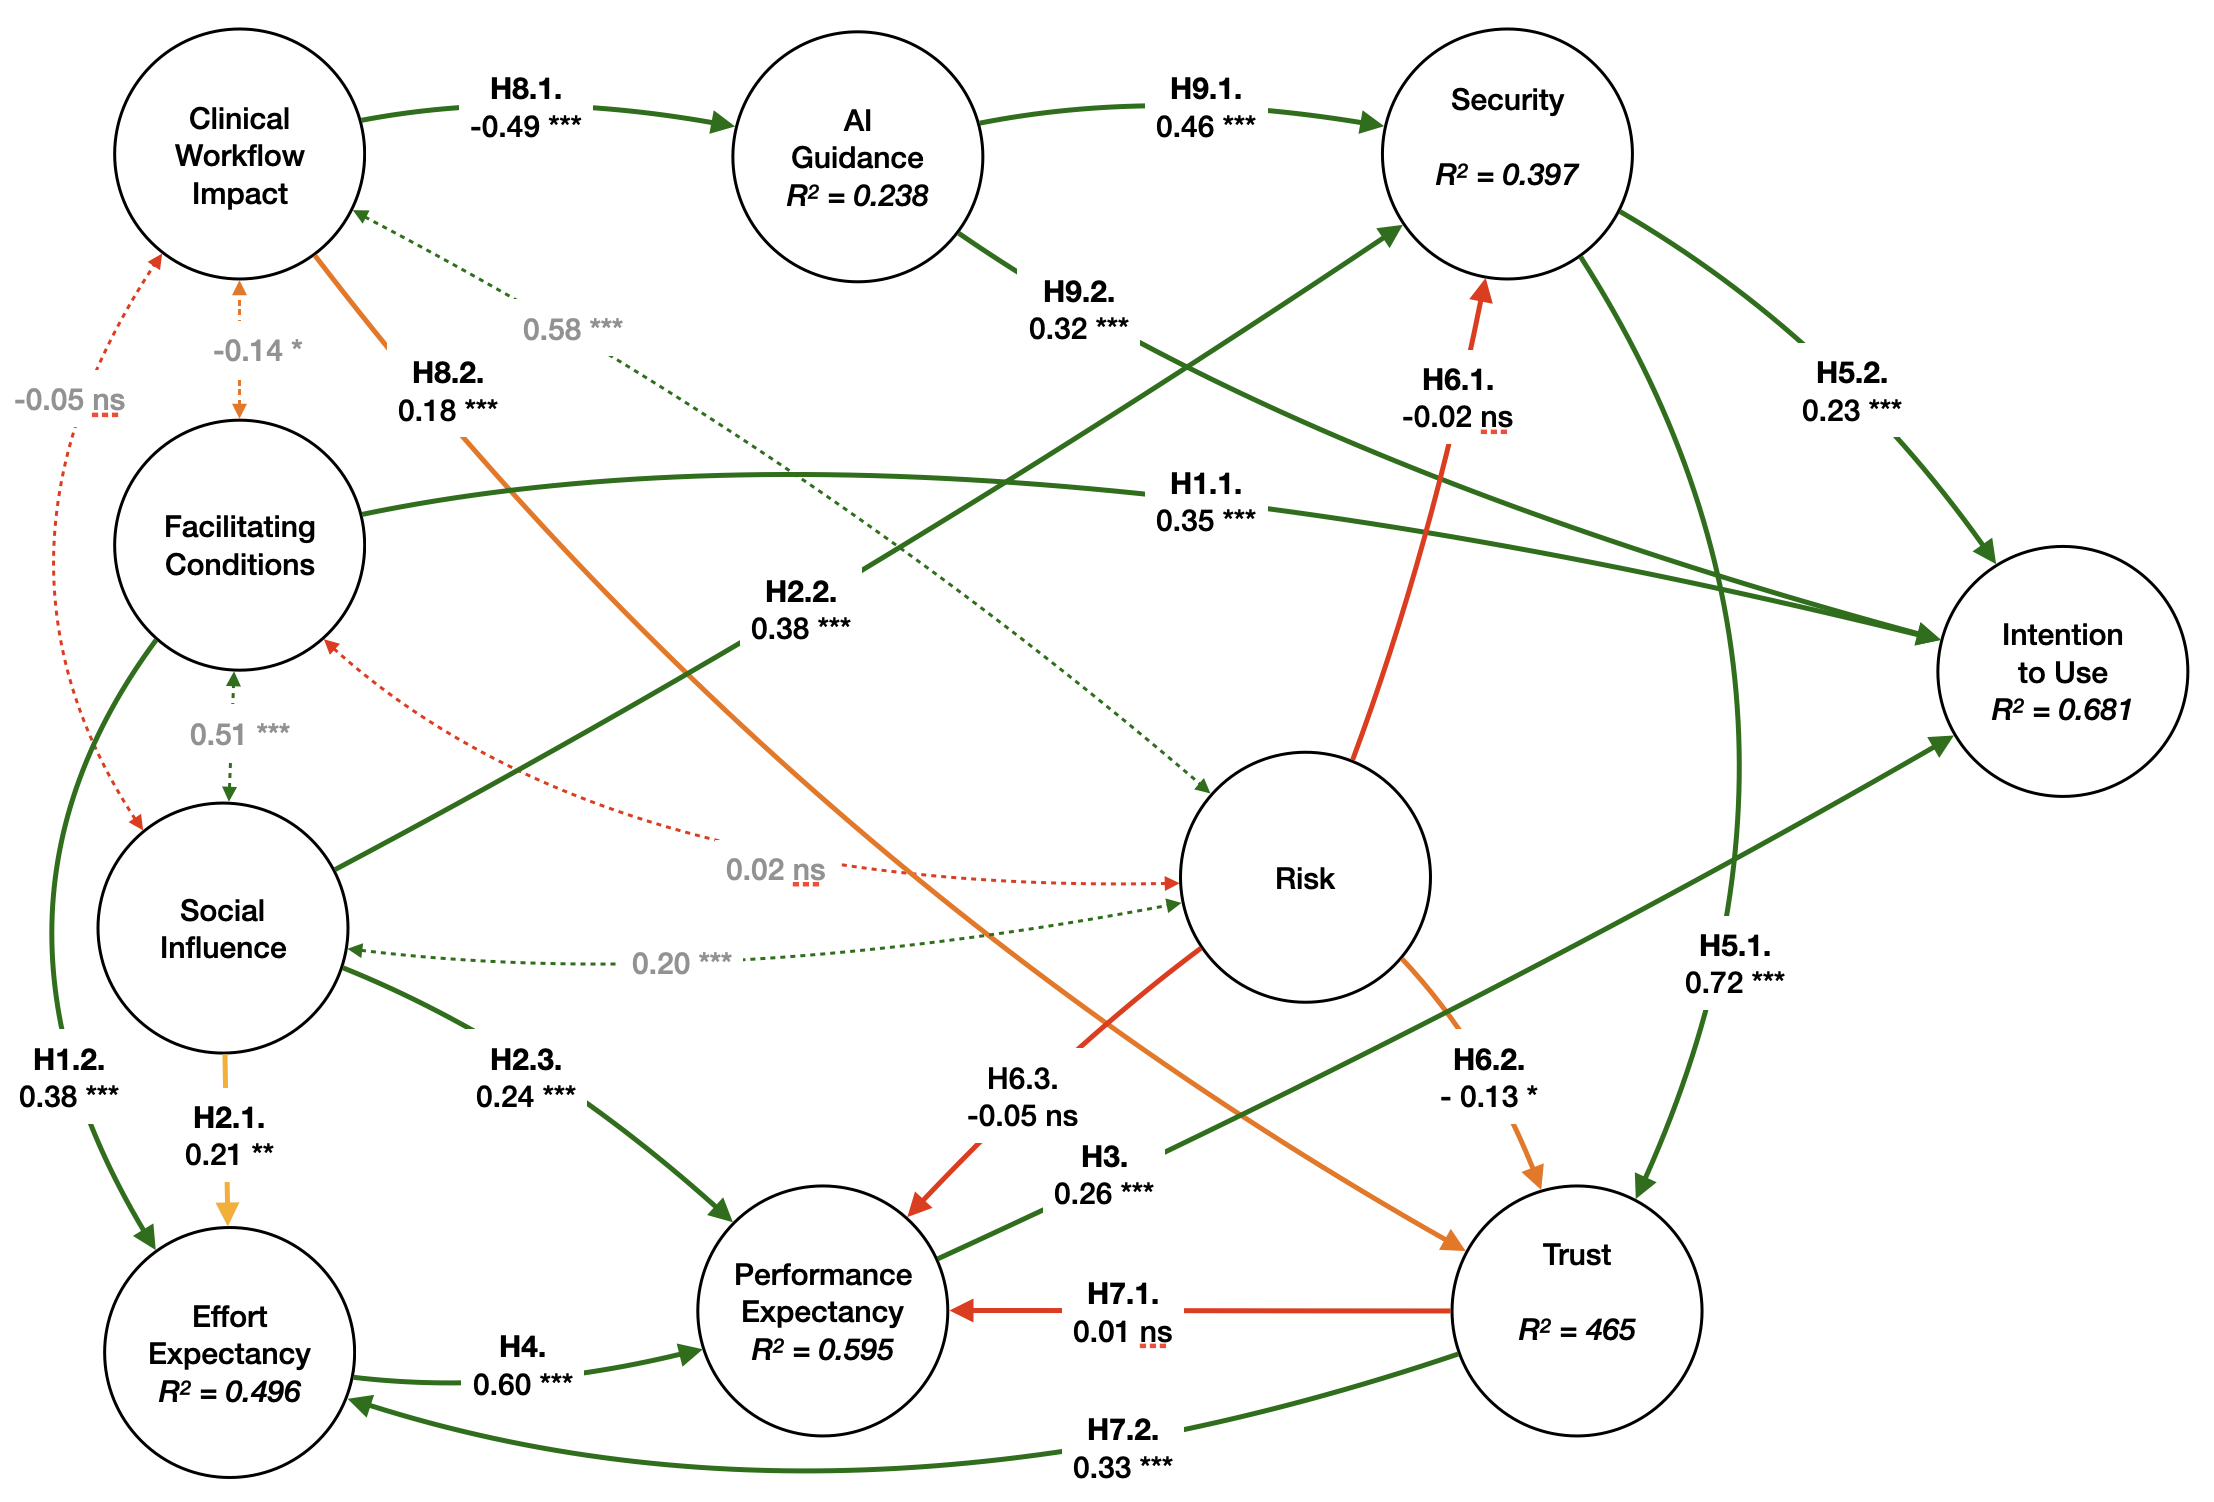
\includegraphics[width=0.794\linewidth]{fig074}
\caption{Detailed results of the research model. For beta results, the significance values are: in green for *** significant at level $\alpha = 0.01$; yellow for ** significant at $\alpha = 0.05$; orange for * significant fixed at $\alpha = 0.10$; and red for \underline{n}ot \underline{s}ignificant (ns).}
\label{fig:fig074}
\end{figure*}
%%%%%%%%%%%%%%%%%%%%%%%%%%%%%%%%%%%%%%%%%%%%%%%%%%%

Effort expectancy is positively affecting the performance expectancy construct ({\bf H4.}).
If clinicians think that AI assistance can provide an easy, clear, and understandable recommendation, they are more likely to expect higher performance from the system.
Theoretically, this adds a new view to UTAUT research.
As the ease of use for intelligent agents increases, performance expectancy for AI systems will become more positive.
Besides, there is a significant decrease in terms of mediating effects for groups of {\it female}, {\it young clinicians}, as well as clinicians with {\it advanced education} and {\it novice knowledge} on the medical imaging practice.
Hence, the AI community should ensure that these intelligent agents cover the above group characteristics.
Not only do our results require intelligent agents to be easy and understandable to use clearly for the majority of clinicians.
But consider the group differences from the mediating effects to introduce AI on the clinical workflow properly.

In our results, security shows a strong effect on clinician's trust ({\bf H5.1.}) toward AI systems. At the same time, a strong impact on specific groups of moderating effects, such as decreasing the groups of {\it females}, {\it young clinicians} with {\it advanced education} but {\it novice knowledge} on medical imaging.
The role of attitude, specifically, becomes more important when we consider the moderating effects of {\it males}, {\it older clinicians}, as well as clinicians in {\it developed countries} with {\it higher education} and {\it expert knowledge}.
The impact of security on attitude and behavioral intention ({\bf H5.2.}) is significant and increased for these groups. At the same time, the research community must consider the adoption of AI in this clinical workflow in the medical imaging domain.

Although some of our hypotheses ({\it e.g.}, {\bf H6.1.} and {\bf H6.3.}) are not supported for perceived risk, our empirical findings demonstrate that perceived risk is an important construct for some groups of the moderating effects.
Perceived risk is related to the level of AI performance ({\bf H6.3.}) concerning clinician's expectations, where the groups of {\it females}, and clinicians working in {\it developed countries} (Table~\ref{tab:tab012}) are showing small, yet, significant values.
It is related to the degree to which clinicians believe using the technology will improve their diagnostic performance and final patient care.
Specifically, it is related to the possibility of AI misdiagnosing a patient and not performing as expected.
Therefore, failing to deliver more accurate decision-making in the clinical workflow.

Perceived trust in patient's privacy ({\bf H6.2.}) is also related to perceived risk, but this time only significant for the groups of {\it female clinicians}.
Here, perceived trust pertains to clinicians' concern over misuse or unwanted disclosure of their patients' information.
Another critical empirical finding of this study is that perceived risk negatively impacts perceived security ({\bf H6.1.}).
Depending on the group of the moderating effects, clinicians would feel insecure using AI if they perceive a low performance of the model and risk their trust in patients' privacy.
From another perspective, the perceived trust of clinicians within this new AI paradigm would increase by improving the algorithm performance and successful implementation of the diagnostic tasks.
The obtained results and insights can serve both AI and HCI communities.

The inclusion of the construct for the clinical workflow impact enabled us to understand if there was a significant but weak impact on trust ({\bf H8.2.}).
Specially, when considering the moderating effects (Table~\ref{tab:tab012}).
Our results show that for some groups ({\it e.g.}, {\it young clinicians} and clinicians with {\it novice knowledge} on the medical imaging field), the clinical workflow impact is not significantly related to their trust in the technology.
According to our results, the same weak link between the influence of trust on performance expectancy ({\bf H7.1.}) and effort expectancy ({\bf H7.2.}), is clear on groups of {\it young} and {\it novice clinicians}.
On the contrary, for the groups of expert clinicians ({\it e.g.}, typically {\it older clinicians} and clinicians with {\it expert knowledge}), the impact of AI on the clinical workflow is significantly related to trust.

Comprehensively, the role of AI guidance on security ({\bf H9.1.}) and behavioral intention ({\bf H9.2.}) retained significant regardless of moderator variables.
However, the new AI guidance construct ({\it i.e.}, the aim of clinicians to follow an AI recommendation) on security ({\bf H9.1.}), decreases with all moderating effects except for {\it males} and {\it older clinicians}.
Similarly, the role of AI guidance on intention to use ({\bf H9.2.}), decreases with all moderating effects. Still, this time except {\it males}, {\it older clinicians}, and clinicians with {\it expert knowledge}.

\subsection{Design Recommendations}
\label{sec:chap004006002}

With the growing demand for intelligent agents in the clinical workflow of medical imaging, our findings can provide valuable guidelines and implications for design.
From the present study, we recommend a new perspective for the design and development of the next generation of AI systems to secure successful implementation of the technology for patient diagnosis.
The present study stressed the critical role of trust in accepting intelligent agents.
As some authors also state~\cite{LIU2022107026}, yet complex solutions, building and maintaining clinicians' trust is a high priority to facilitate user engagement and acceptance.

\vspace{1.50mm}

\noindent
From the following aspects, efforts can be made concerning our design recommendations:

% ####

% Ver aqui:

% https://www.sciencedirect.com/science/article/pii/S0747563221003496?via%3Dihub

% No 5.2. Practical implications

% ####

% Ver aqui:

% https://www.sciencedirect.com/science/article/pii/S0747563221003162?via%3Dihub

% No 8.3. Managerial implications

% ####

% Ver aqui:

% https://www.sciencedirect.com/science/article/pii/S0747563221001631#bib64

% No 6.2. Managerial implications

% ####

\vspace{1.00mm}

\begin{enumerate}
\item An intelligent agent should inform clinicians concerning the consequences of following AI guidance and respective clinical workflow impact for each decision, while providing clinicians control over choice;
\item An AI system should consider demographic data, while adapting the intelligent agent communication depending on gender, age, and country development categories of clinicians;
\item An AI system should take into account the variability of different medical cases, while paying attention to individual conditions and respective needs with varied AI techniques;
\item Designers and developers should enhance the ease of use (usability) and usefulness (functionality) of AI systems to improve perceived security, perceived risk, and trust of clinicians;
\end{enumerate}

\vspace{1.00mm}

Similar to the work of Liu et al.~\cite{LIU2022107026}, our results show how intelligent agents may optimize their control over a decision while informing the consequences of it.
As a (1) first recommendation to introduce an AI algorithm successfully in these clinical workflows, intelligent agents must derive efficient representations ({\it e.g.}, explanations), and use them to specify each patient case.
By providing efficient representations and control, clinicians will trust more AI guidance, with a higher feeling of security and less risk of their decision.

For the (2) second recommendation, our results show how clinicians behave and perceive differently regarding several demographic groups.
We found differences in behavior between gender, age, and country development categories.
Hence, making it essential to adapt the communication of intelligent agents depending on the specific characteristics of each situation.
For example, clinicians from developed countries usually have access to cutting-edge technology and, thus, are more aware of AI technology. However, clinicians from underdeveloped countries are typically less familiar with it.
This is an important finding and recommendation in our study, as the level of AI-based communication must be adapted to groups of clinicians.

As a (3) third recommendation and identical to the last one, we also found that personalizing how intelligent agents report the AI results is an attractive aspect.
AI system designers and developers should consider the variability of different medical cases and embrace the individual needs of clinicians with varied AI techniques.
We must pay attention to individual conditions, such as medical experience ({\it e.g.}, expert {\it vs.} novice knowledge), training levels, and expertise areas.
For instance, expert clinicians may be more susceptible than novice clinicians (and vice versa) to an AI technique trained on a dataset of images or trained with patients' medical histories.

Finally, our (4) fourth recommendation denotes how AI designers and developers should enhance new intelligent agents' usability and functionality.
Although we already reported other salient design recommendations, increasing the ease of use and usefulness of an intelligent agent, respectively, is of chief importance for AI adoption.
Whereas user satisfaction and behavioral intention are consequences of trust~\cite{LIU2022107026, LV2022106993}, ease of use and usefulness are significant antecedents of user's confidence.
By doing so, clinicians' perceived security, risk, and trust towards using the AI system can be largely enhanced.

\subsection{Limitations}
\label{sec:chap004006003}

Despite its contributions, the study has some limitations, and these limitations provide fruitful avenues for further research.
Several of these limitations affect the scope of our results.
Although we had a significant sample of global nationalities, there is still a bias for the small sample size (Table~\ref{tab:tab008}) of specific nationalities.
To understand the effect of this bias, we analyzed the moderator effect of country development categories in our model, which showed the same evidence of invariant measure when compared to other moderators (gender, age, etc.).
However, we did not record race and ethnicity differences in our sample.
Previous works are showing a significant impact of cultural diversity on social influence, usefulness, and behavior intention~\cite{Belanche2019, info:doi/10.2196/27122}.

Another limitation of our study is that it involved clinicians mainly related to radiology.
Given the focus of our study, {\it i.e.}, the medical imaging field, our sample could be biased.
The effect of such characteristics limits the generalizability of this research, since the sample employed in this study could express different perceptions towards AI systems compared to other clinical expertise.
However, the experimental design helps reduce the impact of the Common Method Bias (CMB), which we employed in this study, particularly for the new AI constructs.
Moreover, by combining the survey with outcome variables measured separately and more objectively ({\it e.g.}, frequency of usage/reporting), we are revealing valid results less prone to measurement and method bias.

Despite the above limitations, this study fosters the community understanding of the intention to use AI systems in the clinical workflow. Specifically for the associated constructs of security, risk, and trust concerns on AI systems.
Finally, we provide a valuable set of design guidelines and recommendations for delivering AI systems with these concerns to different user groups.

\subsection{Future Directions}
\label{sec:chap004006004}

Anticipating clinical behavior is notoriously tricky, especially under critical circumstances, such as decision-making in the health sector.
An obvious avenue for future research would be to apply our measurement model to a more broad approach to a higher number of AI applications.
For instance, the applicability of this model to other clinical contexts ({\it e.g.}, systems for clinical drug development, epidemiology, dementia treatment, between others), where decision support systems are also demanding.
Indeed, such a study will sample a more extensive and generalizable achievement of our findings and recommendations.
Therefore, future studies should sample a more significant number of users and compare the differences in various clinical domains.

Our generalized application of the research model would require a data collection process of more clinical characteristics for better thorough validation.
For example, it is also essential to understand the clinical behaviors and needs of public and private health institutions.
Hence, further research would examine change in the importance of constructs over these characteristics, mainly to see the effect of safety, risk, and trust on behavioral intention over different scenarios.
The results of this study should promote future research and consider adding other antecedents of behavioral intention.

\section{Conclusion}
\label{sec:chap004010}

The advent of AI techniques enables intelligent agents as a new medical imaging diagnosis paradigm.
However, the implementation success of these AI techniques depends on clinicians' trust and acceptance of such systems.
The present study examines the role of security, risk, and trust in influencing the acceptance of AI-based assistance.
We empirically tested the proposed research model, showing that trust is a crucial path in shaping user acceptance, which mediated the effects of AI-specific aspects on user acceptance.
Additionally, we demonstrate that clinicians' demographic characteristics are relevant moderators of the relationship between factors and behavioral intention.
Indeed, this study indicates that some characteristics of clinicians should be considered when developing novel intelligent agents for the clinical workflow of medical imaging diagnosis.
The study offers significant findings and implications for better design, development, and implementation of this level of AI-based assistance.

